%%%%%%%%%%%%%%%%%%%%%%%%%%%%%%%%%%%%%%%%%
% Masters/Doctoral Thesis 
% LaTeX Template
% Version 1.43 (17/5/14)
%
% This template has been downloaded from:
% http://www.LaTeXTemplates.com
%
% Original authors:
% Steven Gunn 
% http://users.ecs.soton.ac.uk/srg/softwaretools/document/templates/
% and
% Sunil Patel
% http://www.sunilpatel.co.uk/thesis-template/
%
% License:
% CC BY-NC-SA 3.0 (http://creativecommons.org/licenses/by-nc-sa/3.0/)
%
% Note:
% Make sure to edit document variables in the Thesis.cls file
%
%%%%%%%%%%%%%%%%%%%%%%%%%%%%%%%%%%%%%%%%%

%----------------------------------------------------------------------------------------
%	PACKAGES AND OTHER DOCUMENT CONFIGURATIONS
%----------------------------------------------------------------------------------------

\documentclass[11pt, oneside]{Thesis} % The default font size and one-sided printing (no margin offsets)

\graphicspath{{Pictures/}} % Specifies the directory where pictures are stored

\usepackage[square, numbers, comma, sort&compress]{natbib} % Use the natbib reference package - read up on this to edit the reference style; if you want text (e.g. Smith et al., 2012) for the in-text references (instead of numbers), remove 'numbers' 
\hypersetup{urlcolor=blue, colorlinks=true} % Colors hyperlinks in blue - change to black if annoying
\title{\ttitle} % Defines the thesis title - don't touch this


\begin{document}

\frontmatter % Use roman page numbering style (i, ii, iii, iv...) for the pre-content pages

\setstretch{1.3} % Line spacing of 1.3

% Define the page headers using the FancyHdr package and set up for one-sided printing
\fancyhead{} % Clears all page headers and footers
\rhead{\thepage} % Sets the right side header to show the page number
\lhead{} % Clears the left side page header

\pagestyle{fancy} % Finally, use the "fancy" page style to implement the FancyHdr headers

\newcommand{\HRule}{\rule{\linewidth}{0.5mm}} % New command to make the lines in the title page

% PDF meta-data
\hypersetup{pdftitle={\ttitle}}
\hypersetup{pdfsubject=\subjectname}
\hypersetup{pdfauthor=\authornames}
\hypersetup{pdfkeywords=\keywordnames}

%----------------------------------------------------------------------------------------
%	TITLE PAGE
%----------------------------------------------------------------------------------------

\begin{titlepage}
\begin{center}

\textsc{\LARGE \univname}\\[1.5cm] % University name
 
\begin{figure}[h]
\includegraphics[width=4cm]{Figures/Untitled1}
\centering
\end{figure}

\textsc{\Large Bachelor Thesis}\\[0.5cm] % Thesis type

\HRule \\[0.4cm] % Horizontal line
{\huge \bfseries \ttitle}\\[0.4cm] % Thesis title
\HRule \\[1.5cm] % Horizontal line
 
\begin{minipage}{0.4\textwidth}
\begin{flushleft} \large
\emph{Author:}\\
{\authornames} % Author name - remove the \href bracket to remove the link
\end{flushleft}
\end{minipage}
\begin{minipage}{0.4\textwidth}
\begin{flushright} \large
\emph{Supervisor:} \\
{\supname} % Supervisor name - remove the \href bracket to remove the link  
\end{flushright}
\end{minipage}\\[3cm]
 
%\groupname\\
\deptname\\ % Research group name and department name
 
{\large \today}\\[4cm] % Date
%\includegraphics{Logo} % University/department logo - uncomment to place it
 
\vfill
\end{center}

\end{titlepage}

%----------------------------------------------------------------------------------------
%	DECLARATION PAGE
%	Your institution may give you a different text to place here
%----------------------------------------------------------------------------------------

%\Declaration{

%\addtocontents{toc}{\vspace{1em}} % Add a gap in the Contents, for aesthetics

%I, \authornames, declare that this thesis titled, '\ttitle' and the work presented in it are my own. I confirm that:

%\begin{itemize} 
%\item[\tiny{$\blacksquare$}] This work was done wholly or mainly while in candidature for a research degree at this University.
%\item[\tiny{$\blacksquare$}] Where any part of this thesis has previously been submitted for a degree or any other qualification at this University or any other institution, this has been clearly stated.
%\item[\tiny{$\blacksquare$}] Where I have consulted the published work of others, this is always clearly attributed.
%\item[\tiny{$\blacksquare$}] Where I have quoted from the work of others, the source is always given. With the exception of such quotations, this thesis is entirely my own work.
%\item[\tiny{$\blacksquare$}] I have acknowledged all main sources of help.
%\item[\tiny{$\blacksquare$}] Where the thesis is based on work done by myself jointly with others, I have made clear exactly what was done by others and what I have contributed myself.\\
%\end{itemize}
 
%Signed:\\
%\rule[1em]{25em}{0.5pt} % This prints a line for the signature
 
%Date:\\
%\rule[1em]{25em}{0.5pt} % This prints a line to write the date
%}

\clearpage % Start a new page

%----------------------------------------------------------------------------------------
%	QUOTATION PAGE
%----------------------------------------------------------------------------------------

\pagestyle{empty} % No headers or footers for the following pages

\null\vfill % Add some space to move the quote down the page a bit

\textit{``Be the change you want to see in the world."}

\begin{flushright}
Mahatma Gandhi
\end{flushright}

\vfill\vfill\vfill\vfill\vfill\vfill\null % Add some space at the bottom to position the quote just right

\clearpage % Start a new page

%----------------------------------------------------------------------------------------
%	ABSTRACT PAGE
%----------------------------------------------------------------------------------------

\addtotoc{Abstract} % Add the "Abstract" page entry to the Contents

\abstract{\addtocontents{toc}{\vspace{1em}} % Add a gap in the Contents, for aesthetics

% What is the problem? What if the topic of this Thesis

This Thesis presents a system that allows a social human-interactive robot to be able to actively learn novel stimuli presented to it, expanding its knowledge base. 

The system detects unknown patterns and decides when those patterns are worth being learned by the robot. The system architecture leans on novelty detection algorithms, that serve to implement two steps: first filtering noise entries; and then evaluating if the entries that have passed the noise filter are known by the existing model, or on the contrary, they are novel entries that are worth learning. When a novel entry is identified, the system activates the learning process to update the model with this new data.
 
The novelty detection system is evaluated in the pose learning domain. The dataset is composed by 28 users that teach 3 different poses to the system. In the experiments, we compare the performance of four different novelty detection algorithms for this task. We first evaluate the noise filter by analyzing how many entries from the same pose have to be shown to the robot to pass the filter. The second step is tested training  the system with one of the poses, then evaluating if the algorithms are able to detect test entries from other poses as novel. A third experiment tests our system for detecting in-class novelties. The results show that the performances vary between the novelty detection algorithms. The best performance is achieved by GMM, with a 86$\%$ F score for detecting new poses and a 80$\%$ F score to detect variations within poses. 

This novelty detection system opens the door for robotic systems to be able to act as active learners, making their own decisions about when it is worth to learn from new stimuli. Additionally, to the extent of our knowledge, there is no reference on Novelty Detection for pose recognition in a Human-Robot interactive application, so this work is a novelty itself.  

}

\clearpage % Start a new page

%----------------------------------------------------------------------------------------
%	ACKNOWLEDGEMENTS
%----------------------------------------------------------------------------------------

\setstretch{1.3} % Reset the line-spacing to 1.3 for body text (if it has changed)

\acknowledgements{\addtocontents{toc}{\vspace{1em}} % Add a gap in the Contents, for aesthetics

I would like to express my sincere gratitude to every person who has helped me in my path to finish successfully my Engineering Degree.  

To my Thesis's director, Victor, who has helped me understand and organize the topic of the Thesis. He has also guided my in the research process, and has encouraged and motivated me to see research as a possible career path.

To the Department of Systems Engineering and Automation, and everyone who made possible that my design could be tested.

To all my professors, in Universidad Carlos III de Madrid and in UC Berkeley. They have taught me not only concepts, but a mindset to face life. 

To my friends, who have helped me through the bad and the good times, and who have always believed in me and tried to understand me. Than you for cheering for me.

To my family, for their infinite support and comprehension. None of this would have been possible without you.

\bigskip  ------

Me gustaría expresar mi más sincera gratitud a todas las personas que me han ayudado en el camino a realizar mi grado en Ingeniería.

A mi director de Tesis, Víctor, que me ha ayudado a entender y organizar el tema del trabajo. También me ha guiado en el proceso de investigación, y me ha animado y motivado a ver la investigación como una posibilidad de salida para mi carrera.

Al Departamento de Ingeniería de Sistemas y Automatización, y a todas las personas que han hecho posible que mi diseño se haya podido probar. 

A todos mis profesores en la Universidad Carlos III de Madrid y en UC Berkeley. No solo me han enseñado conceptos, sino también una mentalidad para enfrentarme a la vida. 

A mis amigos, que me han ayudado en lo bueno y en lo malo, y que siempre han creído en mi y han tratado de entenderme. Muchas gracias por los ánimos.

A mi familia, por su apoyo y comprensión infinitas. Nada de esto habría sido posible sin vosotros.   

}
\clearpage % Start a new page

%----------------------------------------------------------------------------------------
%	LIST OF CONTENTS/FIGURES/TABLES PAGES
%----------------------------------------------------------------------------------------

\pagestyle{fancy} % The page style headers have been "empty" all this time, now use the "fancy" headers as defined before to bring them back

\lhead{\emph{Contents}} % Set the left side page header to "Contents"
\tableofcontents % Write out the Table of Contents

\lhead{\emph{List of Figures}} % Set the left side page header to "List of Figures"
\listoffigures % Write out the List of Figures

\lhead{\emph{List of Tables}} % Set the left side page header to "List of Tables"
\listoftables % Write out the List of Tables


%----------------------------------------------------------------------------------------
%	DEFINITIONS
%----------------------------------------------------------------------------------------

\clearpage % Start a new page

\setstretch{1.5} % Set the line spacing to 1.5, this makes the following tables easier to read

\setcounter{chapter}{0}

\chapter{Definitions} % Add the "Abstract" page entry to the Contents

\lhead{\emph{Defintions}} % Set the left side page header to "Abbreviations"

\label{definitions}
\begin{table}[h]
\begin{tabular}{l p{10cm}} % Include a list of Abbreviations (a table of two columns)
\emph{curiosity} & “a strong desire to know and learn something” and “an unusual or interesting object or fact” \cite{oxford}. First mentioned in page \pageref{curiosity}. \\ \\
\emph{novel stimuli} & “different from anything known before; new, interesting and often seeming slightly strange” \cite{Pimentel2014}. First mentioned in page \pageref{novel}. \\ \\
\emph{new data entry} & the data entry has not been presented to the system any time before, defined in page \pageref{new}. \\ \\
\emph{strange data entry} &  data entry that does not conform with the base of knowledge, defined in page \pageref{new}. Opposite to \emph{known data}, defined as data similar to the entries formed by the base of knowledge. \\ \\
\emph{interesting data entry} & data entry that is relevant to understand how the system works, defined in Chapter page \pageref{new}. Opposite to \emph{noise}, defined as meaningless data. \\ \\
\emph{Novelty Detection} & “detecting previously unobserved (emergent, novel) patterns in the data” \cite{Chandola2009}. First mentioned in page \pageref{novelty}.\\ \\
\emph{abnormal or anomalous data} & “data that differs from the data in the training dataset" \cite{Pimentel2014}. Opposite to \emph{normal data}, defined as data that can be predicted by the model of the training set. First mentioned in page \pageref{abnormal}.\\ \\
%\textbf{Acronym} & \textbf{W}hat (it) \textbf{S}tands \textbf{F}or \\

\end{tabular}
\end{table}


\clearpage % Start a new page

%----------------------------------------------------------------------------------------
%	DEFINITIONS
%----------------------------------------------------------------------------------------

%\clearpage % Start a new page

%\lhead{\emph{Definitions}} % Set the left side page header to "Symbols"

%\listofnomenclature{ll} % Include a list of Symbols (a three column table)
%{
%Name & Definition
%\emph{curiosity} & "a strong desire to know and learn something” and "and unusual or interesting object or fact” \cite{oxford} \\
%\emph{novel stimuli} & "different from anything known before; new, interesting and often seeming slightly strange” \cite{Pimentel2014} \\
%\emph{new data entry} & the data entry has not been presented to the system any time before, defined in page 5 \\
%\emph{strange data entry} &  data entry that does not conform with the base of knowledge, defined in page 5 \\
%\emph{interesting data entry} & data entry that is relevant to understand how the system works, defined in page 5 \\
%\emph{Novelty Detection} & “detecting previously unobserved (emergent, novel) patterns in the data” \cite{Chandola2009}\\
%\emph{abnormal data} & "data that differs from the data in the training dataset" \cite{Pimentel2014} \\

%& & \\ % Gap to separate the Roman symbols from the Greek

%$\omega$ & angular frequency & rads$^{-1}$ \\
% Symbol & Name & Unit \\
%}

%----------------------------------------------------------------------------------------
%	DEDICATION
%----------------------------------------------------------------------------------------

\setstretch{1.3} % Return the line spacing back to 1.3

\pagestyle{empty} % Page style needs to be empty for this page

\dedicatory{Dedicado a mis abuelos, que siempre alentaron mi curiosidad

To my grandparents, who always encouraged my curiosity} % Dedication text

\addtocontents{toc}{\vspace{2em}} % Add a gap in the Contents, for aesthetics

%----------------------------------------------------------------------------------------
%	THESIS CONTENT - CHAPTERS
%----------------------------------------------------------------------------------------

\mainmatter % Begin numeric (1,2,3...) page numbering

\pagestyle{fancy} % Return the page headers back to the "fancy" style

% Include the chapters of the thesis as separate files from the Chapters folder
% Uncomment the lines as you write the chapters

% Chapter 1

\chapter{Introduction} % Main chapter title

\label{Chapter1} % For referencing the chapter elsewhere, use \ref{Chapter1} 

\lhead{Chapter 1. \emph{Introduction}} % This is for the header on each page - perhaps a shortened title

%----------------------------------------------------------------------------------------

Imagine you are at the library, studying, and you decide to take a little break. You start observing your friend sitting next to you, and he is reading a book. Suddenly he looks at the girl sitting across you. 'Automatic reflex', you may think, if you think about it at all. But then he looks at her a second time, and a third, and a fourth. Now you are thinking 'What is he doing?' 'Who is she?', and you may even look at the girl yourself.  

Why do we behave like that?  We don't pay attention when unusual things happen once, but we become curious when an unusual thing happens several times.

\label{curiosity}
Curiosity is defined as “a strong desire to know and learn something" and as an “unusual or interesting object or fact" \cite{oxford}. Curiosity means giving importance to what you do not recognize, and wanting to learn about it. This process is inherent in humans and other animals. As toddlers, we are curious about anything new, and we learn by asking questions like 'What is that?' or 'Why is it like that?'. We actively want to know about new and strange things and we want to learn about them, to be able to recognize them the next time.

The process of being curious relies on identifying novel stimuli that are “different from anything known before; new, interesting and often seeming slightly strange” \label{novel} \cite{Pimentel2014} and being able to learn from them, while ignoring stimuli that are already known or seem uninteresting. Therefore, curiosity can imply a desire of learning a new stimuli when it is considered strange and interesting.

In the field of Artificial Intelligence, Machine Learning is the branch that deals with the design and study of mathematical systems that can learn from data. The methods used in Machine Learning have been applied to the field of robotics, enabling robots to learn new abilities. Traditional methods in Machine Learning are based on passive learning. In such learnings, the robot system would create a model from the data in the training phase, and then it would predict a classification for new data in the test phase. However, in most of these methods, inputs are being introduced and analyzed by a human operating the system, therefore, the system is simply a computational tool. Classification is pre-conditioned by the data in the training system, the knowledge base, and it is only be expanded if the human operator includes more data in the training set and the system can relearn. 

In \emph{active learning}, the system itself is an actor in the learning process. The system can understand and decide what is relevant and what is unknown, and it is intrinsically motivated to explore the areas of the learning space that it does not know, ask the user about them and add new data to its knowledge base. Thus, the learning process is directed by the system and is continuous. The system can learn autonomously and interact with the humans to ask for more information if it needs to. Interactive robots are also perceived as more intelligent by humans \cite{Cakmak2010}.

For this purpose, in the development of Machine Learning, this process of curiosity is critical. It constitutes an important component for the effective and long-term operation of intelligent robot systems allowing computationally efficient, unsupervised and incremental exploration and learning of new skills and environments \cite{Nehmzow2013}. This ability means a huge step in their autonomy and learning habits, making them process information more like humans. This is key because it brings us closer to the "holy grail of Artificial Intelligence: general purpose human level intelligence equivalence"\cite{Brooks1990}. 

This Thesis presents a system that allows a human-interactive robot to be able to actively want to learn about novel stimuli presented to it, via a visual system, expanding its knowledge base. The system will be able to detect novel stimuli using machine learning algorithms, analyzing if a stimuli is interesting and different than anything seen before. When a novel stimuli is detected the system learns the data and adds it to its knowledge base. When the stimuli is considered known or not interesting, the system will ignore it. \footnote{The definitions of \emph{new}, \emph{interesting} and \emph{strange} will be further developed in the introduction of Chapter \ref{Chapter2}.}

The general learning performance of the system is based on ignoring perceptions that are already known, and highlighting novel stimulus.  This concept is based of what is called habituation, and is inspired on biological systems. Habituation is a “type of non-associative learning used to describe the behavioral phenomenon of decreased responsiveness of a cognitive organism to a recently and frequently presented stimulus”, and it has been observed in a number of biological organisms \cite{Nehmzow2013}.  

There is an specific field of Machine Learning that deals with this problem, called Novelty Detection \cite{Chandola2009}. It is applied in situations where you have the task of classifying test data that differs in some aspects from the data that are available during training \cite{Pimentel2014}. It can be defined as “detecting previously unobserved (emergent, novel) patterns in the data”, and incorporating these novel patterns into the normal model afterwards \cite{Chandola2009}. Classification algorithms of different origins and types are used for this purpose. In this Thesis, the performance of different novelty detection algorithms for this specific problem are analyzed.

The developed system has been tested in an experiment which consisted of several people posing in front of a RGB-D (Red, Green, Blue, Depth) camera, such as the Kinect.
\begin{figure}[h]
\includegraphics[width=4cm]{Figures/Example1}
\centering
\caption{Example of a 3D representation of the skeleton shape data retrieved from the Kinect \label{fig:ske}}
\end{figure}


A kinect module locates the 3D position of the user's joints, and retrieves set of data representing a “skeleton” shape of the data, such as the one in Figure \ref{fig:ske}. In Chapter \ref{Chapter4}, this process will be further explained.

After the trained is finished, the system is able to detect when the new users are posing in a different way than the previous users, and it will be able to learn that novel pose.

\section{Objectives}

The aim of this Thesis is to design a system that is able to:


\begin{description}

  \item[Distinguish between what is known and what is strange] \hfill \newline
The system will have to identify when a new entry of data is different from anything known before and alert about it. If the entry is detected as already known or not interesting, the program will have to ignore it. It is important to highlight that we cannot consider a \emph{right} way of posing, but a \emph{learned} way of posing. New instances will be tested against these \emph{learned} instances.

\clearpage
  \item[Identify when an entry is interesting] \hfill \\
If, in the example opening the thesis, we asked our friend about any new move he does, we would bother him. If he scratches his arm, or drops the pencil or stretches, all this moves will be strange to us, but if we ask him every time 'What are you doing?' he would think that we are crazy. We are not interested in asking him unless the event has happened frequently enough to be interesting.

To imitate human behavior, the system will have to distinguish between when a new entry is detected as different because it is noise, meaning that the camera was not able to record it properly, it was a one-time event, or because it is a novel entry.

  \item[Learn from novel data] \hfill \\
The system, after detecting a novel entry, will have to add it to its knowledge base. Thus, a mechanism needs to be established to incorporate these interesting and strange entries in a continuous way. 

The detection of novel poses is the main objective of the Thesis, implying that the system will need to be able to alert the user of this event, so that we can check that the system is operating correctly. After alerting, the system can ask the user 'What are you doing?' or whatever the experiment require. 

\item[Aim to have a high detection rate while keeping the false alarm rate low] \hfill \\
  The program will aim to identify as many novel entries as possible, while ignoring as many known or uninteresting entries as possible. This means that the program has to avoid false alarms, so it will not bother the interacting user unnecessarily. 

  \item[Have an autonomous behavior and display information] \hfill \\
The system will need to do this active learning tasks autonomously. To check the correct operation of the system, some kind of user interface will need to be built to display the system information, such as when a new pose is detected as novel.

While establishing a human-robot, visual or voice, interaction is out of the scope of this Thesis, we will need to define mechanisms that allow our system to transmit information to other interaction modules created by the research group where this Thesis was developed. This implies creating an alert system that can transmit this information.  


\end{description}

\clearpage
\section{Organization, structure of the document}

This document is organized as follows. Chapter \ref{Chapter2} introduces the formal definition of the problem and the machine learning algorithms used to address it. Chapter \ref{Chapter3} describes proposed solution as the software architecture and is followed by the results of the testing of the software with real data in different experiments in Chapter \ref{Chapter4}. Chapter \ref{Chapter5} presents an overview of the methods an approaches used in related work. Finally, Chapter \ref{Chapter6} summarizes the main contributions and describes future work and opened issues worth studying.

\begin{flushright}

\end{flushright}

% Chapter 2

\chapter{Problem Definition} % Main chapter title

\label{Chapter2} % For referencing the chapter elsewhere, use \ref{Chapter1} 

\lhead{Chapter 2. \emph{Problem Definition}} % This is for the header on each page - perhaps a shortened title

%----------------------------------------------------------------------------------------
This Thesis addresses the problem of creating a system that allows a human-interactive robot to actively want to learn about novel stumuli presented to it, expanding its knowledge base. Thus, this Thesis deals with the problem of giving a machine the ability of being curious.

Novel stimuli are defined as “different from anything known before; new, interesting and often seeming slightly strange” \cite{Pimentel2014}. We have to identify three aspects of the data; \emph{new}, as not seen anytime before, \emph{interesting}, and \emph{strange}. 

\textbf{New} means that the data entry has not been presented to the system any time before. This aspect will be a characteristic of the data entry itself. \label{new}

\textbf{Strange} data entries are those that do not conform with the base of knowledge, it will be opposite to \emph{known data}. Whereas the aspec \emph{new} refers to the data themselves, \emph{strange} is a prediction made by the model about the data, this prediction is further explained in Section \ref{2.1}. 
Imagine a user poses in front of the camera, every time the user moves and the system records a pose, it will be new. However, the system may classify this new pose as \emph{strange} or \emph{known}, and this is a prediction made by the system, and is subject to the systems performance and accuracy. \label{strange}. The opposite, \emph{known data}, according to the system, is similar to the entries formed by the base of knowledge.

\textbf{Interesting} can be defined as relevant to understand how the system works \cite{Chandola2009}, it is opposite to \emph{noise} An interesting entry has the potential to make our model change or update. The aspect \textbf{interesting} will be directly related to the frequency of appearance of the stimuli. It will also be a prediction made by the model about the data, and  is further explained in Section \ref{2.2}.  For example, similarly to the example proposed in the Introduction of the Thesis in page 1, if the system asked our friend every time he looked to a new girl, our friend would be very annoyed. However, it the system only asked our friend when he looked more than three times to the same girl, probably that girl is interesting to our friend. \label{interesting}. The opposite, \emph{noise} or \emph{noisy data}, is defined as meaningless data.

The following sections expand more these concepts and divide the problem definition in smaller parts:

Section 2.1 Quantifying the strangeness of a stimuli \\
Section 2.2 Quantifying the interest of a stimuli \\
Section 2.3 Learning from novel stimuli \\
Section 2.4 Controlling the curiosity level \\
Section 2.5 Working autonomously and being interactive 
  

\section{Quantifying the strangeness of a stimuli} \label{2.1}

The field of Machine Learning that deals with this task is called \emph{Novelty Detection}. It can be defined as “detecting previously unobserved (emergent, novel) patterns in the data”  \cite{Chandola2009}. \label{novelty}

Typical classification and pattern recognition in Machine Learning deals with two or more classes. The algorithms create a model that is composed of examples from these classes. Then, when presented with a new entry, the algorithms give an estimate of the class this new entry belongs to. 

Novelty detection, instead, tries to detect (or identify) \emph{abnormal data}. That is, data that differs from the data in the training dataset\label{abnormal}. It has become very popular in applications with the need of identifying abnormal behavior. These applications include failure detection in industrial systems, or mass-like structures in mammograms \cite{Pimentel2014}. All this systems have in common that their complexity leads to a limited understanding of a direct identification between a cause and a consequence of what is \emph{normal} and \emph{abnormal}. The problem is that the set of \emph{abnormal} examples is very under-sampled compared with the \emph{normal} set, and also there is a large number of possible \emph{abnormal}  and \emph{normal} modes. In some of the applications there is a high cost of obtaining examples of \emph{abnormal behavior}, for example in industrial damage, to obtain a new abnormal instance one machine has to be broken on purpose, with its associated cost.

This results in typical Machine Learning classification not being suited for these applications. There are not enough examples to create a \emph{normal} class and an \emph{abnormal} class, and there could be multiple unidentified \emph{abnormal} classes.

The approach used by Novelty Detection is a one-class classification. One class, the positive \emph{normal} class must be distinguished from all other possibilities. The positive class must be, then, very well sampled, while the negative \emph{abnormal} classes can be under-sampled. Figure \ref{fig:one} illustrates a 2D representation of a one-class classifier learned from the normal instances, and how anomalies are those instances that are outside the one-class classifier boundary.

\begin{figure}[h]
\includegraphics[width=8cm]{Figures/Oneclass}
\centering
\caption[One class Novelty Detection]{One class Novelty Detection. Retrieved from \citeauthor{Chandola2009} \cite{Chandola2009}. \label{fig:one}}
\end{figure}

In the case of the experiment in this Thesis, there are many poses that the user can adopt. It would limit the learning potential of the system to just learn a limited number of the poses and classify the new entries according to them. Instead, the intention of this Thesis if that the system can learn an unlimited number of poses from the user and that the system has the thrive to learn new poses.

The formal approach in Novelty detention is creating a large one-class model of “normality”, formed by as many examples representing normal instances as possible. The new entries are tested against this model of normality, as in Figure \ref{fig:one}, resulting in some sort of \emph{novelty score}. In the case of the figure, \emph{anomalies} would have a high novelty score, while the normal instances inside the boundary would have a low novelty score.

The model of normality is represented as M(\( \theta  \)), where \( \theta  \)
representing the free parameters of the model. This model is used to assign a novelty score, $z(x)$, to test data $x$. A higher novelty score will represent a more \emph{abnormal} instance.

The classification of \emph{normal} or \emph{abnormal} is obtained after comparing the novelty score with a threshold $k$. If:

\begin{equation}
	z(x) \geq  k 
\end{equation}

Then $x$ is classified as \emph{abnormal}. The equation was retreived from \citeauthor{Pimentel2014} \cite{Pimentel2014}.

Different types of models M, methods for setting their parameters \( \theta  \), and methods for determining novelty thresholds $k$ have been proposed in the literature. The classification and further explanation of the Novelty Dectection techniques used will be developed in Section \ref{3.6}.

\label{thresholds}

In \textbf{state-space novelty detection} approaches, the cross-entropy between the normal and the new distributions can be computed. The threshold is set by maximum cross-entropy value computed between the entire training set and each time-series in the training set. Each new entry will be considered normal if its cross-entropy is lower than the values of the entries in the training set \cite{Pimentel2014}.

In \textbf{probabilistic novelty detection} techinques, a novelty threshold may be set yaking into account where the most extreme samples generated from the normal distribution will lie. For example in GMM based algorithms, the threshold is set to be the minimum log likelihood of the training data \cite{Pimentel2014}.

In \textbf{distance based novelty detection} approaches, the distances to the one class centroid for all points in the same scene are computed, and a threshold based on the mean and standard deviation of the distances of the normal instances instances is determined \cite{Pimentel2014}. On other words, if the new point is futher that the average of the training data to the centroid, then its abnormal. 

The methods applied to calculate the threshold in this Thesis are explained in Sections \ref{thres1} and \ref{thres2}.
 
\section{Quantifying the interest of a stimuli} \label{2.2}

The interest of the stimuli is related to classifying the stimuli as interesting or noise. Noise can be defined as a phenomenon in data which is not of interest to the analyst \cite{Chandola2009}. The problem relies in that a noise entry is also an \emph{strange} entry, and will be classified as such. An entry can be detected as strange because it is noise or because it is an novelty, whiwh impies that is interesting by definition. We need to have a filter to separate these two cases, we are only interested learning an entr if it is novel, not if it is noise. We are not interested in adding noise to our model of normality, because that will distrub future novelty detections and may lead to misclassifications.

\begin{figure}[h]
\includegraphics[width=8cm]{Figures/Outliers}
\centering
\caption[Novel and noise entries in 2D.]{Novel and noise entries in 2D. Retrieved from \citeauthor{Chandola2009} \cite{Chandola2009}. \label{fig:out}}
\end{figure}

In Figure \ref{fig:out}, N1 and N2 represent normal data, already added to the model of normality in the one-class classification. 
All instances O1, O2 and O3 will be classified as abnormal, because their novelty score with  be higher than the threshold defined. The difference is that O3 happens more frequently than the other two. This means that we consider O3 more interesting.
The interestingness level may also have a threshold, and the frequency needed for the stimuli to be considered interesting may be changed.

The interest of an stimuli will be directly related to the frequency of appearance of the stimuli with respect to all of the data received by the system up to that point. An application to the “frequent episode discovery problem” in temporal data mining is presented in \cite{frequency}. For a pre-defined confidence level, upper and lower thresholds for the observed frequency of an event can be determined \cite{Pimentel2014}, which can be used to decide whether the event can be considered interesting or noise.

An example of noisy and interesting entries in the experiment this Thesis deals with would be depicted in Figure \ref{fig:noise}.

\begin{figure}[!htb]
\minipage{0.5\textwidth}
  \includegraphics[width=5cm]{Figures/Noise}
  \centering
\endminipage\hfill
\minipage{0.5\textwidth}%
  \includegraphics[width=5cm]{Figures/Normal}
  \centering
\endminipage
  \caption{Examples of noisy and insteresting entries in the experiment of pose recognition. \label{fig:noise}}
\end{figure}

Noise in this case would be entries that have been badly recorded by the Kinect, this is further explained in Section \ref{4.2}. In this case, a noisy entry is that where the legs are crossed, because the Kinect could not identify them correctly, and that probably some of the other joints were not recorded properly either. We would expect a noise entry to happen rarely, while the interesting entry will be the type of data we will record frequently.

The idea behind noise detection is that noise is defined to happen very rarely. As mentioned in the previous section, noise is under-sampled with respect to the rest of the data. As can be seen in Figure \ref{fig:out}, interesting events tend to form clusters in the knowledge space, when they are repeated in time in a small area. While noise has a more uniform distribution trougout space, with much less density. There is also a necessity of detecting if a lot of noisy entries are being recorded, because that can mean that there is something wrong with the camera or the processing of the data, and we may need to fix it. So, if a lot of noisy entries are being recorded, then it becomes an interesting event, and thus a novel event. 

As in the previous step, we will need to determine a interest threshold, and compare the interestingness score of the new data with the rest of the entries received. But in this case, the interest threshold is computed from all the entries presented to the system ever, instead of just the model of normality. As we can see in the figure, the interest of the stimuli is determined when taking into account all entries, not just the model of normality. We need to take into account all entries from O3, in Figure \ref{fig:out}, to determine that there is a group of entries that is becoming interesting in that point.  

Thus, the system needs to keep record of two sets of data:

\begin{itemize}

\item A dataset consisting of all the instances every received, including those that have been received but not added to the normal model. This dataset is used to check if the new entries have formed any cluster with previous recorded data, if they are becoming interesting.

\item The normal set, that trains the normality model. Serves to check if the interesting entries are novel or, on the other hand, are something that our system already knows.

\end{itemize}

\section{Learning from novel stimuli}

The last step, after identifying a new stimuli as strange and interesting, is incorporating it to the normal model. This step means adding the entry to the set of data considered as “normal” and recalculating the model for the one-class classification, thus recalculating the threshold values for the novelty score and the frequency of appearance for interesting entries.

This means that when a new stimuli, similar to the previous novel stimuli, is showed to the system, it will now be identified as interesting and normal, as known. 

The approach is based on cumulative learning, because the system accumulates the learned novel poses, expanding continuously its normality model. There are many open challenges related with long-term operation of this system and constraints such as dynamically expandable learning structures and bad learning. We have to deal with the decision of whether to further expand the model when a new perception is misclassified, which may lead to future errors in the learning process. 

This also happens in biological systems, when a baby is taught that an apple is called “pear”, she will identify all future apples as pears, and she will think that she knows the concept when someone mentions a pear to her.

\section{Controlling the curiosity level}

The parameters of the curiosity level of the robot must also be controllable. The programmer is able to choose if the robot is very curious or not.
This is directly related to controlling the novel score threshold and the frequency of appearance for interesting entries. This control will be done by means of a graphic interface where the programmer will be able to tune these parameters.

This aspect is key for the customization of the learning process. Depending on the application, or on the experiment, we may want the system to be very curious or less curious. In our case, we have the objective of not bothering the interacting user too much, but in an application such as video survaillance, probably we want to alert as soon as someone is detected in the camera.

\section{Working autonomously and being interactive}

The system does these active learning tasks autonomously. This means that the retrieval of the data and the computation of the classifications must be fast. The programming will be done using Python and specific Machine Learning libraries, these libraries are referenced in Sections \ref{3.6} and \ref{4.3}.

Altought, was mentioned before, the interaction part is out of the scope of this Thesis, the system needs an interface to communicate to the programmer the outcome of the predictions. Thus, it needs to have a graphic interface to show the results, raise alerts and accept input information from the user.

The only way of going further novelty detection, and deepen in the learning and human-interactive process of the system is asking the user when a novel entry is detected. It is, then, necessary to establish mechanism to display the outcomes from the system to other interactive modules that can actually do the work of interacting with the user. The system needs to provide information about \emph{when} to ask the user.

\begin{flushright}

\end{flushright}
 
% Chapter 3

\chapter{Description of the proposed solution} % Main chapter title

\label{Chapter3} % For referencing the chapter elsewhere, use \ref{Chapter1} 

\lhead{Chapter 3. \emph{Description of the proposed solution}} % This is for the header on each page - perhaps a shortened title

%----------------------------------------------------------------------------------------

This chapter describes the proposed solution. The developed system needs to be able to complete each of the steps stated in the Problem Definition. The system general functioning scheme includes the proposed solutions for all the steps, and is depicted in Figure \ref{fig:scheme}  It will be explained in detail trough the sections in this Chapter. 

The classification of the data in this Chapter is based on the definitions of \emph{new}, \emph{strange} and \emph{interesting}. proposed in page \pageref{definitions}, and that were further developed in \pageref{new}.

\begin{figure}[h]
\includegraphics[width=10cm]{Figures/Esquema}
\centering
\caption[System general scheme functioning.]{System general scheme functioning. The new entry is first tested to be classified as interesting or noise. If it is interesting, it is then tested to check if it is strange, resulting in an interesting novelty, or if it is known. Noisy and know entries are discarded, while novelties are learned \label{fig:scheme}.}
\end{figure}

The process begins with the arrival of a new pose data from the modules of the Kinect. That entry is tested against all other data entries received up to that point. If the result is positive, then the entry is considered interesting, as defined in page 5. After that, the entry is be tested against the knowledge base to determine if it is strange, again as defined in page 5. If the result is positive in this second test, the entry is classified as novelty, raising the alerts to the programmer and to other learning modules. The entry is then learned by the system by adding it to the knowledge base.   

If the new pose data is regarded as not interesting it is classified as noise, and it is just kept in the dataset of all entries received. If it is regarded as not strange, it is classified as known and is also kept in the dataset of all entries received. After the new data is classified and added to the correspondent dataset, the system waits for the arrival of another new pose data.     

Not to waste computational resources, the system checks first if the new data is interesting instead of strange. The reason behind this is that it would not make sense to use time and computational power in checking if a data entry is strange, if it is later detected as not interesting. With this structure, the system filters first the data so we can get rid of noisy entries in the first step, and it does not make extra computations unnecessarily. 

The steps presented in the previous section can be identified in Figure \ref{fig:scheme} as well. Quantifying the interest of the stimuli is represented as the decision 'interesting?' and quantifying the strangeness is identified in the decision 'strange?'. Learning from novel stimuli is depicted as the process 'learn pose' after the pose is detected as novel. Working autonomously is related with the functioning system working in a continuous loop; and being interactive involves that the results of \emph{noise}, \emph{known} and \emph{novelty} should be transmitted to the user. Note that the curiosity level is the threshold that determines the answers for the decisions 'interesting?' and 'strange?', as there are two tests and the paramenters considered for each one are different, the system needs two curiosity levels.

The designed solution for each of the steps independently will now be explained in detail in the following sections. Altought the general scheme involves first the noise filtering step and then the strangeness evaluation, the sections present first the strangness evalutation and then the noise filtering. This is because the strangeness evaluation method is more intuitive, and helps to understand concepts that will be later used in the noise filtering method.

\section{Enabling the system to evaluate the strangeness of a stimuli} \label{3.1}

The step of quantifying the strangeness of a stimuli allows the system to identify the new data entry as known or novelty. In Figure \ref{fig:sche_strange} the process is located in the general scheme of the system. 

\begin{figure}[h]
\includegraphics[width=9cm]{Figures/Esquema_strange}
\centering
\caption{Strangeness evaluation step located in the general scheme. \label{fig:sche_strange}}
\end{figure}

This process, as mentioned in Section \ref{2.1}, consists on obtaining the model of normality M(\( \theta  \)), where \( \theta  \)
representing the free parameters of the model. Then this model is used to assign a novelty score, $z(x)$, to new data $x$. 

Some novelty detection methods predict directly a label, \emph{normal} or \emph{abnormal}, when a new entry is detected. Some others provide an score of how well a entry fits into the model. In this later cases, from the model of normality, we can obtain a novelty threshold. This will be further explained in the following sub-sections.

The following rule applies, where $z$ is the novelty score of a new instance $x$ and $k$ is the novelty threshold.:
\medskip

\begin{equation}
	z(x) \geq  k 
\end{equation}

If this condition holds, then $x$ is considered as \emph{abnormal}. This equation was retreived from \cite{Pimentel2014}. 

\subsection{Model of normality}

The normal dataset consists of the poses that have been considered normal and were learned at some point. The model of normality is generated by the novelty detection algorithms, using the normal set as the training set. The algorithms used in this Thesis are explained in Section \ref{3.6}. The normal set is expanded as the system learns new poses. The system learns whatever the user teaches it. We consider that the learned poses are a consistent base of knowledge. 

\subsection{Obtaining the novelty score}

The model is obtained using one-class classification methods. These classifications methods allow to compute an score of how well each instance fits the calculated model. The score is calculated differently for the distinct methods used in this Thesis, how these methods operate will be further explained in Section \ref{3.6}.

If we consider the normal dataset N1, and fit a model $M$ with these entries:
\medskip

\centerline{$ N_1 = [n_1, n_2, n_3,...,n_m]  $ and $ M(N_1)$ }

We can obtain a fitting score, from the algorithm, for each of the instances from the model $ M(N1) $ :
\medskip

\centerline{$ scores = [z(n_1), z(n_2), z(n_3),...,z(n_m)] $}

This set of scores represents a distribution of the scores of the normal entries. This distribution can be normalized, as shown in Figure \ref{fig:normal_d}, obtaining a mean $\mu$ and a standard deviation $\sigma$. 

\begin{figure}[h]
\includegraphics[width=15cm]{Figures/Normal_d}
\centering
\caption[Normal distribution]{Normal distribution, including Standard Deviation and Z score parameters. Retrieved from Wikipedia \cite{standard}. \label{fig:normal_d}}
\end{figure}

A standard score\footnote{The standard score formula can also be denominated the normal score or z score in the literature} of a new entry, $o_1$ \footnote{The convention is using the letter $o$ to label outliers}, can be calculated as follows:

\begin{equation}
standard.score(o_1) = \dfrac{z(o_1) - \mu}{ \sigma}
\end{equation}

Since the distribution is symmetrical, we are interested in the absolute value of this standard score. This is our final $novelty$ $score$.

\begin{equation}
novelty.score(o_1) = abs( \dfrac{z(o_1) - \mu}{ \sigma})
\end{equation}

\subsection{Obtaining the strangeness threshold} \label{3.1.3}

\label{thres1}

The $strangeness$ $threshold$ is obtained from the scores of the normal dataset. We are using the Extreme Value Theorem (EVT) to obtain its value. EVT is a "branch of statistics which deals with extreme deviations of a probability distribution" \cite{Pimentel2014}. It considers extremely large or small values in the tails of the distribution that is assumed to generate the data to obtain the threshold. \cite{Pimentel2014}. This approach can be applied to both \textbf{distance based novelty detection} \textbf{probabilistic novelty detection}, as mentioned in Section \ref{thresholds}.

For example, consider that the novelty threshold is located at one sigma units distance from the mean of the scores in the normal set. Thus, in Figure \ref{fig:normal_sig} can be observed that the strangeness threshold in standard score, also known as z score, for a value of 1 $\sigma$, would be  -1 and 1, where the limits are drawn. Any entry with an score outside the red are will be considered outside the threshold, and thus, abnormal. 

\begin{figure}[h]
\includegraphics[width=15cm]{Figures/Normal_d_sigma}
\centering
\caption[Normal distribution for one sigma]{Normal distribution for one sigma. The area in red corresponds to the scores in the distribution that are less than 1 sigma units away from the average. Modified and retrieved from Wikipedia \cite{standard}. \label{fig:normal_sig}}
\end{figure}

The equation that represents entries outside the red region is:

\begin{equation}
1 \geq abs( \dfrac{z(o_1) - \mu}{ \sigma} )
\end{equation}

Expading the equation:

\begin{equation}
\begin{split}
z(o_1) \geq \mu +\sigma \\
z(o_1) \leq \mu -\sigma
\end{split}
\end{equation}

In this example, the score of the new data entry is one time $\sigma$ units away from the average value, $\mu$ of the normal scores. A value of one $\sigma$ means that, a new entry is labeled as \emph{normal} if lays within the 68\% of the closests scores to the mean of the dataset. If the standard score is higher than 1, the score $z(o_1)$ can be considered high with respect to 68\% of the normal entries, and it can be classified as strange. 

Imagine we now use a threshold $+K$ and $-K$, instead of +1 and -1. 

\begin{equation}
novelty.score(o_1) = abs( \dfrac{z(o_1) - \mu}{ \sigma})
\end{equation}

\begin{equation}
K \geq abs( \dfrac{z(o_1) - \mu}{ \sigma} )
\end{equation}

If we develop this expression:

\begin{equation}
1 \geq abs( \dfrac{z(o_1) - \mu}{ K \times \sigma} )
\end{equation}

\begin{equation}
\begin{split}
z(o_1) \geq \mu + K \times \sigma \\
z(o_1) \leq \mu - K \times \sigma
\end{split}
\end{equation}

Thus, the standard score for the different entries is inversely proportional to the units of standard deviation, $\sigma$, we consider for the \emph{normal} entries. By increasing the units of sigma considered, we could lower all standard scores, an thus, we would consider as \emph{normal} those scores that were before close to the threshold. 

In consequence, the normalized score can be modified by multiplying the value of $\sigma$ times a K factor, increasing the units of sigma considered. While we can maintain a novelty threshold of +1 and -1.


\section{Enabling the system to filter noise by evaluating the interest of a stimuli} \label{3.2}

The step of quantification of the interest of a stimuli will allows the system to identify the new data entry as noise or interesting. And thus, it is key in the process of detecting and discarding unwanted noise. In Figure \ref{fig:sche_interest} the process is located in the general scheme of the system. 

\begin{figure}[h]
\includegraphics[width=9cm]{Figures/Esquema_interest}
\centering
\caption{Interest evaluation step located in the general scheme. \label{fig:sche_interest}}
\end{figure}

The interestingness of a new data entry depends on what the system has seen before, if it has seen 1000 very similar entries, and 1 new entry is slightly different, probably it will be considered noise. But it also depends on the application, maybe the system needs to be very sensitive to this 1 different entry, and we do not want to discard it. Thus, the system needs to account for all the entries it has ever seen, to see patterns of repetition, and needs to customize its sensitivity. It is important to remember that we are interested in finding out when to ask the user when the system finds something novel, and the application may need that the system does not bother the user too much, so the sensitivity should be low, or on the other hand, we want the system to ask the user a lot, so the sensitivity should be high.

This step can be approached from different perspectives. It can be considered as an outlier detection problem, only that we are interested in detecting when a data entry stops being an outlier and starts being interesting. It can also be considered a clustering problem, in which the objective would be finding out when the data starts forming a cluster around a point, because that would mean that the frequency of appearance around a point is high, and therefore, indicating that this point it is not mere noise but, instead, an interesting data point. 

We can consider all the data ever presented to the system as \emph{normal} in a one-class classification, with a base of knowledge of all the seen entries. Then we can apply a novelty detection method and find a novelty score for new data using the Extreme Value Theorem (EVT). When the data is labeled as \emph{normal}, then it is similar to something that has happened before, it happens frequently enough to be considered interesting. Depending of the novelty detection algorithm used, we will be using the different approaches mentioned in the previous paragraph. 

Figure \ref{fig:plot_out} show this process for One-class classification in a 2D reduction:

In the \textbf{subfigure (a)} we observe the initial dataset, with only one event happening frequently around an area. This event is what we consider the normal knowledge base.

In the second \textbf{subfigure} \textbf{(b)}, we have added new events that happens frequently around an area, and they have formed a new cluster. We now see two clusters of white points, the new cluster of points can be see in the center left side of the image. The model has been recalculated, taking into account all the instances, that are the normal and the new clusters and the outliers. This is the process we follow to evaluate interestingness. We can see how the one class classification applied to all data changes from (a) to (b). In (b), the new cluster is inside the threshold line of the one class classification. This means that the event happens frequently enough to be considered in the one class classification model, modifying it, and thus is interesting. As it is interesting, the system now evaluates the strangeness of the cluster, as explained in the general scheme, Figure \ref{fig:scheme}. 

In the third \textbf{subfigure (c)}, we evaluate the strangenness of the cluster. We build the one class classification model with only the white, normal instances from (a), as explained in Section \ref{3.1}. It can be observed that the new cluster event, in black, is now outside the threshold, and thus, it is considered strange. As the cluster is classified as  \emph{interesting and strange}, the system concludes that it is, indeed, a \emph{novelty}. Detecting a novelty is what sets off the alert to the learning system and to other interaction modules to ask the user about it. The new events are not noise and are cannot be detected as known by the system, so it wants to learn about them to increase the knowledge base and be able to recognize them in the future. 

\begin{figure}[!htb]
\includegraphics[width=6cm]{Figures/one_class/a}
\centering
\\[\baselineskip]
\minipage{0.5\textwidth}
  \includegraphics[width=6cm]{Figures/one_class/b}
  \centering
\endminipage\hfill
\minipage{0.5\textwidth}%
  \includegraphics[width=6cm]{Figures/one_class/c}
    \centering
\endminipage\hfill
 
\caption[Plot of outlier detection in One-class classification]{Plot of outlier detection in One-class classification. (a) represents the initial dataset, (b) we have added new events that formed cluster, the plot represents the insterestingness evaluation, computing a model that takes into account all instances. The new event is inside the threshold, it is interesting (c) resprsents the strangeness evaluation test, the model is trained only with the normal instances from (a), the new event cluster is outside the thresold formed by the normal instances, it is considered strange. Example adapted from Scikit-Learn webpage \cite{scikit-learn}. \label{fig:plot_out}}
\end{figure}

This means that both steps, quantifying the strangeness and the interest of a stimuli can be solved with similar novelty detection processes and algorithms, only using different bases of knowledge.

\subsection{Model of normality}

The base of knowledge dataset will consist of all the poses ever presented to the system. The model of normality will be computed from this dataset.

\medskip

\centerline{ $ M(all.instances)$ formed by $ all.instances = [i_1, i_2, i_3,..., i_m]  $  }

The dataset will be expanded every time a new pose is presented to the system.

\subsection{Obtaining the noise score}

To differentiate it from the novelty score, we will name the score obtained to classify the entries as 'interesting' the $noise$ $ score$. If the entry is interesting, then it will have a low noise score.

We can obtain a fitting score, according to the algorithm, for each of the instances from the model $ M(all.instances) $ :
\medskip

\centerline{$ scores = [z(i_1), z(i_2), z(i_3),..., z(i_m)] $}

This set of scores represents a distribution of the scores of all entries. This distribution can be normalized, again as shown in Figure \ref{fig:normal_d}, obtaining a mean $\mu$ and a standard deviation $\sigma$.

Following the same procedure as in the previous section, we can obtain a standardized noise score.
 
\begin{equation}
noise.score(o_1) = abs( \dfrac{z(o1) - \mu}{ \sigma})
\end{equation}
 
\subsection{Obtaining the noise threshold} 

\label{thres2}

Following the same procedure as in subsection \ref{3.1.3}, we can obtain the formula:

\begin{equation}
noise.score(o_1) = abs( \dfrac{z(o_1) - \mu}{ K \times \sigma})
\end{equation}

This K factor, representing the units of standar deviation , $\sigma$, considered.

As seen in subsection \ref{3.1.3} we can declare 1 as the threshold for the noise score.

\section{Enabling the system to control the curiosity level} \label{3.3}

In the formula used to calculate the strangeness and noise score in Equation 3.6 and 3.10:

\begin{equation}
strangeness.score(o_1) = abs( \dfrac{z(o_1) - \mu}{ K \times \sigma})
\end{equation}

The value of K represents where we place the extreme values in the scores of the normal set, the threshold. If we develp the expression, it also represents the units of sigma considered, simplifiyng the threshold to a values of 1. By increasing the value of K, we increase the range fo the extreme values as shown in Figure \ref{fig:normal_d}. Table \ref{tab:sigma} summarizes the percentage of normal scores considered, and where we consider the extreme value, depending on the value of K.

\begin{table}[h]
    \begin{tabular}{ c  c }
    K value & Percentage \\ \hline
    1 & 68 $ \% $ \\ 
    1.98 & 95 $ \% $ \\ 
    2.58 & 99 $ \% $ \\ 
    \end{tabular}
    \centering
    \caption[Change in the percentage of normal scores considered depending on the value of K multiplying $\sigma$]{Change in the percentage of normal scores considered depending on the value of K multiplying $\sigma$, as presented in Figure \ref{fig:normal_d} \label{tab:sigma}.}
\end{table}


This K factor, as we have seen, can be applied to both strangeness and interestingness evaluation. We have named it the $curiosity$ $ factor$, and will serve as a way to modify the novelty score threshold. This is key to the sensityvity of the system. We can increase the sensitivity by decreasing the curiosity factor, because, to be normal, the new score will need to be very close to the mean with respect to all other instances in the base of knowledge.

As the value of the $cusiosity$ $factor$ depends on the sensitivity degree we want to achieve, and also on the nature of the data in te application, it needs to be commputed empirically.

\section{Enabling the system to learn from novel stimuli}

\begin{figure}[h]
\includegraphics[width=9cm]{Figures/Esquema_learn}
\centering
\caption{Learning step located in the general scheme. \label{fig:scheme_learn}}
\end{figure}

The step of learning from novel stimuli is placed right after the data is classified as a \emph{novelty}, as seen in \ref{fig:scheme_learn}. The process consists of adding the novel data to the base of knowledge, the normal data set. After that, the Model of normality must be recalculated and expanded. A new score will be added to the set of normal scores and the mean $\mu$ and the standard deviation $\sigma$ will de recalculated as well.

A key concept in this step is avoiding misclassification. Building a model on misclassification can lead to future errors in the learning process. This can be avoided by asking the user when a novel entry is detected. By doing this, we can also ask for a label for the pose. The system will tell the user 'I don't know what you are doing. What are you doing?'. This confirmation will also be helpful to calculate the false alarm and the detection rate of the system. As mentioned before, the interaction with the user is out of the scope of this Thesis. However, the interface of the system has a 'Learn pose' button that allows the programmer to decide which poses to learn.

\section{Enabling the system to work autonomously and to be interactive}

The last step in building the system is that all this presented solutions have to be integrated in a system that works autonomously. Figure \ref{arch} displays the proposed software and hardware architecture for the system. It is important to remember that this process is a continuous closed loop, as shown in Figure \ref{fig:scheme}. In the architecture we only show the flow of data, so the closed loop is not explicitly drawn, since it means only waiting for a new input entry.

\begin{figure}[h]
\includegraphics[width=14cm]{Figures/architecture}
\centering
\caption[System software and hardware proposed architecture]{System software and hardware proposed architecture\label{arch}. The skeleton-shape entry from the modules of the Kinect is preprocessed and saved in the \emph{all instances} dataset. It is then tested for interestingness and strangeness, and the results are displayed to the programmer. If the entry passes both tests, the system has found and novelty and alerts the programmer and other modules of interaction to ask the user. The programmer chooses to learn or not the novel pose by the button input 'Learn pose', that leads to saving that novel pose in the \emph{normal instances} dataset, learning it. When either of the satasets is updated, the corresponding model is updated as well.}
\end{figure}

The process starts with the Kinect recording the user, and retrieving a skeleton-shape entry using a Kinematic extraction module. This work was already done in the Department of Systems Engineering in a previous project \cite{Gonzalez-Pacheco2013}. This entry, $I$, will be then preprocessed, so it can be analyzed by our system and it is saved in the \emph{all instances} dataset. The nex step, is that $I$ is tested against the constructed interestingness model to analyze if it is interesting. The intestetingness score is displayed to the user via a simple interface. If $I$ passes the test and is interesting, it is tested against the normal model, to verify if it is strange. The outcome of this second test is displayed to the user too. If $I$ passes both tests, it means that the entry is a novelty. The following step is communicating an alert to other modules, if necessary. The programmer is responsible of deciding if the system must learn the pose, via a button in the interface. The pose is learned by storing it in the \emph{normal instances} dataset. The models are reconstructed when the corresponding datasets change, for future operation. 

In future iterations of the system, the learning step will not need to be supervised by the programmer. This supervision is only temporal, and serves to monitor the operation of the system in this first version built for the Thesis. Also, the integration with other modules os interaction is an area of future work.

\section{Description of the used novelty detection methods} \label{3.6}

Novelty detection techniques can be classified in the following categories, according to \cite{Pimentel2014}: 
(i) probabilistic, (ii) distance-based, (iii) reconstruction-based, (iv) domain- based, and (v) information-theoretic techniques. \cite{Pimentel2014}. Each category has a series of advantages and disadvantages, and different computational costs. Since, there is no single universal method for novelty detection \cite{Nehmzow2013}, the choice if the appropiate algorithm depends on the task. In the Experiments Chapter, four algorithms have been chosen to test their novelty detection performance for the pose recongnition problem adressed. This section describes the algorithms chose. 

\subsection{Probabilistic-based novelty detection methods}

These techniques use probabilistic methods that often involve a density estimation of the \emph{normal}  class. An entry in a low density area indicate that there is probability of it being a \emph{normal}  object \cite{Pimentel2014}.

The method used in this category is \textbf{Gaussian Mixture Model}, a GMM.
A GMM is a probabilistic model that assumes all the data points are generated from a mixture of a finite number of Gaussian distributions with unknown parameters \cite{scikit-learn}.

This Thesis used the implementation of GMM provided by Scikit-Learn Library \cite{scikit-learn}. It does not provide  directly a \emph{normal} or \emph{abnormal} method, but it does provide a built-in function called $score$. The score represents the log probability of a sample under the model. 

\subsection{Distance-based novelty detection methods}

This category includes the concepts of nearest-neighbour and clustering analysis that have also been used in classification problems. It assumes that \emph{normal}  data are tightly clustered, while novel data occur far from their nearest neighbours. \cite{Pimentel2014}

This thesis tested one method from this category, \textbf{K-Means}. The K-means algorithm clusters data by trying to separate samples in n groups of equal variance, minimizing a criterion known as the ‘inertia’ of the groups. \cite{scikit-learn} This algorithm requires the number of clusters to be specified, in this case, as we are interested in a one-class classification, the number of clusters will be 1. The K-means algorithm aims to choose centroids C that minimize the within cluster sum of squares objective function with a dataset X with n samples \cite{scikit-learn}.

The K-means method was also implemented in the the Scikit Learn Library \cite{scikit-learn}. It does not provide a \emph{normal} or \emph{abnormal} label either. The score function in this case represents the opposite of the value of X on the K-means objective \cite{scikit-learn}.

\subsection{Domain-based novelty detection methods}

Algorithms in this category use domain-based methods to characterize the data for the model of normality. These methods typically try to describe a domain containing \emph{normal}  data by defining a boundary around the \emph{normal} class such that it follows the distribution of the data \cite{Pimentel2014}.

Methods used from this category are specifically categorized as "oultier detection methods", and provide directly a label categorizing test data as \emph{normal} or \emph{abnormal}.

One of the algorithms chosen was \textbf{One Class SVM}, from the Scikit Learn Library\cite{scikit-learn}. The One-Class SVM has been introduced to decide whether a new observation belongs to the same distribution as exiting observations (it is an inlier), or should be considered as different (it is an outlier). It requires the choice of a kernel and a scalar parameter to define a frontier. The RBF kernel is usually chosen although there exist no exact formula or algorithm to set its bandwidth parameter. This is the default in the scikit-learn implementation. The $\nu$ parameter, also known as the margin of the One-Class SVM, corresponds to the probability of finding a new, but regular, observation outside the frontier \cite{scikit-learn}.

The other algorithm used is \textbf{Least Squares Anomaly Detection}. It is a flexible, fast, probabilistic method for calculating outlier scores on test data, given training examples of inliers. The model is controlled by two parameters: sigma (a kernel length scale, controlling how 'smooth' the result should be) and rho (a regularisation parameter, which controls the sensitivity to outliers) \cite{lsa}. It was implemented by John Quinn from Makerere University, Uganda.

\begin{flushright}

\end{flushright}
% Chapter 4

\chapter{Experiments} % Main chapter title

\label{Chapter4} % For referencing the chapter elsewhere, use \ref{Chapter1} 

\lhead{Chapter 4. \emph{Experiments}} % This is for the header on each page - perhaps a shortened title

This chapter describes the experiments carried out to evaluate the proposed solution. 
 
\section{Description of the dataset} \label{4.1}

The data provided for the evaluation of the system comes from another experiment developed in the Department of Automation and Systems Engineering at Universidad Carlos III de Madrid in the field of gesture and pose recognition \cite{Gonzalez-Pacheco2013}. It consisted of 24 users who taught the robot a predetermined set of poses using a Microsoft Kinect camera, the data retrieved was then labeled by the user trough a voice interaction with the user. Figure \ref{fig:scen} shows the disposition of the experiment. It consisted of a Kinect camera placed inside the Social Robot Maggie \cite{maggie}, in the figure the cone represents the field of view of the Kinect sensor. The user was allowed to move inside the rectangle.

\begin{figure}[h]
\includegraphics[width=7cm]{Figures/Scenario}
\centering
\caption{Scenario of the experiment. Retrieved from \cite{Gonzalez-Pacheco2013}. \label{fig:scen}}
\end{figure}

The data retrieved from the user is a set of parameters that represent the 3D position of 15 joints of a human skeleton. The disposition of the data is showed in Figure \ref{fig:kine}. The entries of the dataset have the following shape:

\begin{figure}[h]
\includegraphics[width=8cm]{Figures/Skeleton}
\centering
\caption{Kinematic of the human body. Retrieved from \cite{Gonzalez-Pacheco2013}- \label{fig:kine}}
\end{figure}
 
Each instance I is a set of $t$ the time stamp sequence number, $u$ the user ID, $J$ the set of joints and $L$ the label of the entry.\label{eq-4.1}
\begin{equation} 
I = (t,u,J,L)
\end{equation}
Each set of joints is formed by 15 joints, that can be seen in Figure \ref{fig:kine}.\label{eq-4.2}
\begin{equation} 
J = (j_1,j_2,...,j_15) 
\end{equation}
Each of the joints is formed by x,y,z 3D positions, qx,qy,qz,qw, orientations and a confidence C.\label{eq-4.3}
\begin{equation} 
j_i = (x,y,z,qx,qy,qz,qw,C) 
\end{equation}

The experiment was subdivided in 3 sets of poses taught to the robot:

\begin{description}
\item[Set 1] consisted in teaching the robot if the trainer was turned to his/her own left, right or if he/she was turned toward the robot.
\item[Set 2] consisted in teaching the robot if the trainer was looking to his/her own left, right or forward.
\item[Set 3]consisted in teaching the robot if the trainer was pointing at his/her own left, right or forward. Example shown in Figure \ref{fig:set3}.
\end{description}

\section{Data treatment for this experiment} \label{4.2}

The data used for this Thesis was extracted from Set 3 of the experiment mentioned in Section \ref{4.1}, where users pointed right, left and forward. In Figure \ref{fig:set3}, picture (a) is an example of a user pointing \emph{left}, in (b) the user is pointing \emph{forward} and in (c) the user is pointing \emph{right}.

\begin{figure}[h]
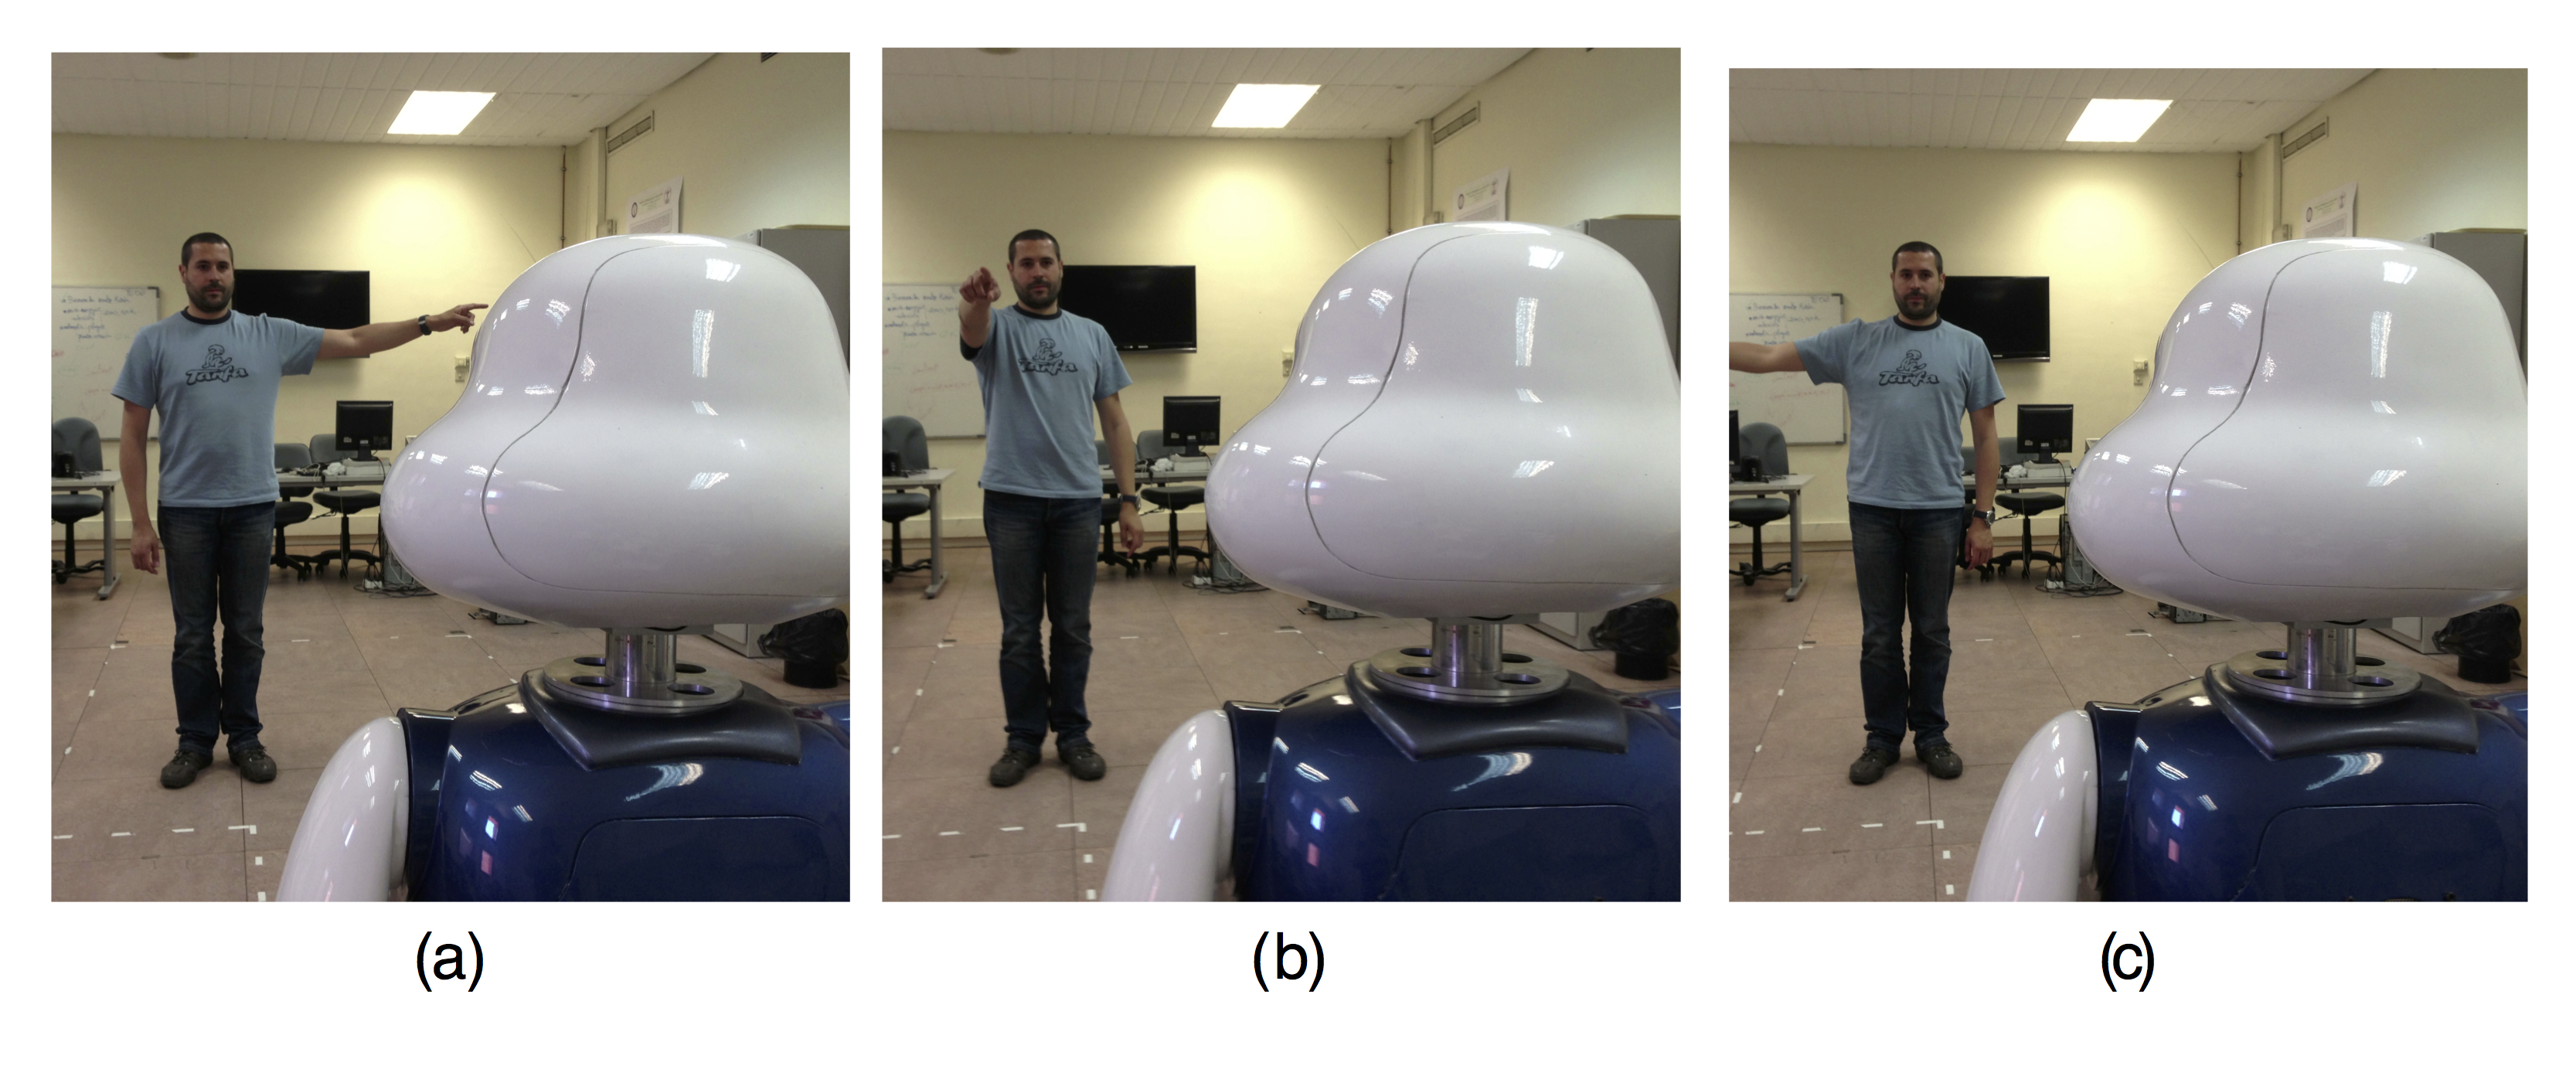
\includegraphics[width=13cm]{Figures/Set3}
\centering
\caption{Photo example of a user pointing. Retrieved \cite{Gonzalez-Pacheco2013}. \label{fig:set3}}
\end{figure}

The users were free to point in the way they preferred. This led to a variety of combinations of arms and positions for the same pose. In Figure \ref{fig:poses} shows examples of users pointing. The color gray represents users posing forward, color blue represents users pointing left, and color green represents users pointing right. 

\begin{figure}[h]
\includegraphics[width=8.5cm]{Figures/Poses}
\centering
\caption[Examples of how different users pointed during the training for pointing poses.]{Examples of how different users pointed during the training for pointing poses. Gray represents users posing forward, blue represents users pointing left, and green represents users pointing right.  Retrieved form \cite{Gonzalez-Pacheco2013}. \label{fig:poses}}
\end{figure}

Each direction at which the users were pointing was labelled as a learning class: \emph{pointing right}, \emph{pointing left} and \emph{pointing forward}. Within each class, there are different subclasses depending on the combinations of arms. In the tables in Appendix A all the combinations and the users that present them are exposed.

The experiment consists in showing the system these examples one by one. The system is able to detect if they belong to different classes by itself, and it learns those new classes when detected. 

However, first we had to understand the problem by observing the data we were dealing with. The work in this Thesis, consisted in initially analyzing these datasets for the purpose of applying novelty detection on them, and then performing such experiments. 

The first question presented is if this data is linearly separable. Using Principal Component Analysis \footnote{PCA is a "statistical procedure that uses an orthogonal transformation to convert a set of observations of possibly correlated variables into a set of values of linearly uncorrelated variables called principal components" \cite{pca}}, all the examples were reduced to 2 dimensions and plotted, as can be seen in Figure \ref{fig:exp03}. Red dots represent users pointing \emph{right}, green dots represent users pointing \emph{forward} and blue dots represent users pointing \emph{left}. The datasets are not linearly separable in 2D.

\begin{figure}[h]
\includegraphics[width=14cm]{Figures/exp03}
\centering
\caption{2D reduction for the pointing dataset with original data. \label{fig:exp03}}
\end{figure}

Observing the different skeletons, we could see that the position of the legs was also very diverse. Because of the location of the Kinect camera, from a low position with respect to the torso and looking upwards, the legs in some users could not be recorded properly. This provoked that some of the entries of the dataset do not have legs at all of the legs appear distorted. Using a One-Class SVM outlier detection, we could confirm that the outliers detected furthest form the frontier were those with legs not recorded properly. Also, the center of the torso of the users was not always recorded at the position (0,0,0), as can be seen in Figure \ref{fig:origin_poses}. The frame of reference used was the Kinect's. For that reason, if different users did not locate at the exact same spot, the x,y,z location of their joints would differ.

\begin{figure}[h]
\includegraphics[width=4.5cm]{Figures/origin_poses}
\centering
\caption[Original data referenced to the Kinect's frame of reference]{Original data referenced to the Kinect's frame of reference. The users moved when recording the poses, so each skeleton was located in a different point. The novelty detection system is more sensible to the differences in the skeleton location than to the pose. red: \emph{pointing right}, green \emph{pointing forward} blue: \emph{pointing left}. \label{fig:origin_poses}}
\end{figure}

Since we are interested in finding differences in the data, this led to the data being very different because of the legs or because of the reference of the torso. Those are not the differences we are interested in, we want the data to be different because it represents pointing each of the three poses. Thus, we need all of the poses to have the same frame of reference. To accomplish this, the torso was moved to the point (0,0,0) and  all the other joints were normalized with respect to the torso. Figure \ref{fig:origin_poses_mod} shows the skeletons shape after the normalization.

\begin{figure}[h]
\includegraphics[width=4.5cm]{Figures/origin_poses_mod}
\centering
\caption[Original data with torso referenced to (0,0,0)]{Original data with torso referenced to (0,0,0). Now all the skeleton's joints are normalized with respect to the torso, located in the origin. red: \emph{pointing right}, green \emph{pointing forward} blue: \emph{pointing left}. \label{fig:origin_poses_mod}}
\end{figure}

The parts of the body that are pore representative of the pointing pose are mostly the arms and the torso, since the users titled their shoulders to point. Thus, we decided to get rid of the legs and hips data points for each user, removing 9 joints: right and left foot, right and left knee and right and left hip. Figure \label{fig:pca} shows the PCA reduction after the modification of the data.

\begin{figure}[h]
\includegraphics[width=14cm]{Figures/exp03_centered}
\centering
\caption{2D reduction for the pointing dataset with modified data. \label{fig:pca}}
\end{figure}

We still cannot separate each of the 3 types of poses linearly. The areas of interest, where the problems may appear, are those where two or more poses merge. 

The final dataset used for the experiments has the following parameters:

\begin{description}
\item[Size]: 87 instances \\ 29 users, 3 instances each, \emph{pointing right}, \emph{pointing forward} and  \emph{pointing left}
\item[Dimensionality]: 81 parameters \\ 9 remaining joints with 8 attributes each $ji = (x,y,z,qx,qy,qz,qw,C)$
\end{description}

\section{Method} \label{4.3}

The data with the poses was provided in .arff files \cite{arff}. Each file consisted of the set of skeletons produced by one user in a session of the experiment mentioned in Section \ref{4.1}. The number of entries of data was different for each user, and it depended on the time that user was recorded. The average number of entries for each user was 218, with a standard deviation of 182. 

The data shape of the data was described in equations \ref{eq-4.1}, \ref{eq-4.2} and \ref{eq-4.3}.

Each entry was formed by $t$ the time stamp, $u$ the user ID, $J$ the set of 15 joints, with 8 attributes each, and $L$ the label of the entry, being \emph{stand pointing right}, \emph{stand pointing left} and \emph{stand pointing forward}. The total number of columns was 124.

A preprocessing step was carried out. It consisted in cleaning the irrelevant columns. These include the label, user-id, h-stamp and all columns corresponding to the position of feet, knees, and hips. The final entries had 81 columns. The data is divided by user and by pose. Each entry represents an user pointing in one of the three directions.

The  novelty detection system uses four algorithms, GMM, One class SVM and K-means, from the Scikit-Learn Machine Learning Library \cite{scikit-learn}, and  Least Squares Anomaly Detection (LSA), that was developed by Jonh Quinn \cite{lsa}. LSA implementation file can be found in his webpage. 

The experiments were carried out with Python \cite{python} programming in a IPython notebook \cite{ipython}. All the experimental data and scripts that were written for this thesis are public and can be accessed in \cite{github}. The IPython notebook was also published in nbviewer \cite{notebook}.The representation of the data was done using the python library Matplotlib\cite{matplotlib}. Other python libraries used for the treatment of the data were Pandas\cite{pandas} and Numpy\cite{numpy}.

\section{Experimental setup}

The system had to be tested with different experiments to demonstrate the accomplishment of the different objectives fo the Thesis. 

1. Firstly, we had to test that the system is able to filter noise. This means that it has to recognize a new pose as \emph{interesting} when it has seen similar poses happen frequently before it, and ignore the entry when it is detected as \emph{noise}. We tested what was the frequency that made the poses become interesting.

2. Secondly, we had to test the performance of the different algorithms to recognize strange entries in the data. The performance was measured training the system with entries only from one pose, e.g. \emph{pointing right}, and testing the system with entries from the same pose and from the other two poses. The entries from the same pose should be detected as \emph{known} and the entries from other poses should be detected as \emph{strange}

\subsection{Algorithms used} \label{4.4.1}

The algorithms used for the experiments are One class SVM, LSA, K-means and GMM.

\textbf{One class SVM and LSA} algorithms provide directly a label that classifies the entries as anomalous or normal. We have translated this labels to the numerical system (1, 0). An entry is assigned a novelty score of 1 when it is detected as anomalous, and a novelty score 0 when it is detected as normal. In the noise filter, a novelty score of 1 is obtained for noisy entries, and a 0 for interesting entries. In the strangeness evaluation test, a 1 is achieved for strange entries, and a 0 for known data. 

\begin{table}[h]
    \begin{tabular}{ c c c c}
    \hline
    Label from the algorithm & Novelty score for the entry $x$ & Noise filter & Strangeness test \\ 
    \hline
    anomalous & 1 & noise & strange \\
    normal & 0 & interesting & known \\
    \hline
    \end{tabular}
    \centering
    \caption[One Class SVM and LSA label interpretation]{One Class SVM and LSA label, for and extry $x$, translation to the binary system. The meaning of the binary novelty scores in the noise filter corresponds to the third column. The fourth column represents the outcome of the binary novelty scores in the strangeness test.}
\end{table}  


\textbf{K-means and GMM} provide a fitting score, the corresponding novelty score calculation from the fitting score was explained in Sections \ref{3.1} and \ref{3.2}. When the novelty score for an entry is lower than 1, the entry is classified as normal and when it is higher than 1 it is classified as anomalous. As mentioned in Section \ref{3.3}, these novelty scores can be tuned depending on the sensitivity desired, with the \emph{curiosity factor}. In the noise filter, a novelty score higher than 1 is obtained for noisy entries, and lower than 1 for interesting entries. In the strangeness evaluation test, a higher than one score is achieved for strange entries, and lower than 1 for known data.

\begin{table}[h]
    \begin{tabular}{ c c c}
    \hline
    Novelty score for the entry $x$ & Noise filter & Strangeness test \\ 
    \hline
    novelty.score(x) $\geq$ 1 & noise & strange \\
    novelty.score(x) $<$ 1 & interesting & known \\
    \hline
    \end{tabular}
    \centering
    \caption[K-means and GMM novelty score interpretation]{K-means and GMM novelty score interpretation for and entry $x$ to the interestingness and strangeness tests. The meaning of novelty score in the noise filter corresponds to the third column. The fourth column represents the outcome of novelty score in the strangeness test.}
\end{table}

An entry that is classified as both \emph{interesting} and \emph{strange}, is considered a \emph{novelty}.

\subsection{Graphic Interface}

A graphic interface was created to show the results of the tests and the shape of the skeletons we were considering, it can be seen in Figure \ref{fig:graphic}.

\begin{figure}[h]
\includegraphics[width=15cm]{Figures/results_imp/right_vs_left1}
\includegraphics[width=15cm]{Figures/results_imp/right_vs_left2}
\includegraphics[width=15cm]{Figures/results_imp/right_vs_left3}
\centering
\caption[Graphic interface]{Graphic interface for the experiments showing, in the right side, the interestingness test of new \emph{pointing left} entries with a base of knowledge of \emph{pointing right} entries. \label{fig:graphic}}
\end{figure}

In the Figure \ref{fig:graphic} we can see the interestingness tests on the left side, the 3D plot corresponds with the representation of the 3D data of the skeletons, and the bar plot representing the noise scores computed for the entry in black. The higher the noise score, the less interesting the entry is to the system. While the noise score is higher than or equal to 1, the entry analyzed is seen as noise, and we do not want to know anything else from it. The bars in this case will be painted red for a visual alert. However, if the noise score is lower than 1, that means that the entry is interesting, and the system wants to pay attention to it, the bars for in this case will be green. 

On the right side, the strangeness test is presented. Once the new entry has passed the noise filter, and thus has been detected as interesting, the system wants to find out if it is part of a known class, or if it is a strange class it has never seen before. If the strangeness score is higher than or equal than 1, the entry is predicted as strange, and thus, as it was interesting and now is algo strange, we can say that it is a novelty, according to its definition in the \textbf{Definitions} section. With this result, the bars are colored green, since the system detected what is the objetive of this Thesis, a novelty. If the strangeness score is less than 1, it means that the entry is a known entry, entries like it are already known by the system, and the bars are colored red. Table \ref{tab:color} summarizes all these cases. 

The Figure \ref{fig:graphic} shows how in each row we showed a new \emph{pointing left} entry to the system. All of the entries added to the system accumulate to calculate the noise score of the new entry, as explained in Section \ref{3.2}. The two first rows show that the entries ponting left are considered noise, as the noise score is higher than 1. However, when we add the third \emph{pointing left} entry, the noise scores lower and are now lower than 1, the system has found that \emph{pointing left} happen frequently, and that it should pay attention to them. Then, it allows the strangeness test to take part. This follows the general scheme we designed in Chapter \ref{Chapter3} and can be seen in Figure \ref{fig:int}. 

\begin{table}[h]
    \begin{tabular}{ c c c c c}
    \hline
    Noise score & Color bar noise & Strangeness score & Color bar strange. & Entry pred. \\ 
    \hline
    $\geq$ 1 & red & - & - & noise\\
    $<$ 1 & green & $<$ 1 & red & known\\
    $<$ 1 & green & $\geq$ 1 & green & novelty\\
    \hline
    \end{tabular}
    \centering
    \caption[Color code for the interface]{ Color code for the interface depending on the noise score and the strangeness score of an entry. \label{tab:color}}
\end{table}

\section{Results}

\subsection{Part 1. Noise filtering by interestingness evaluation}

Figure \ref{fig:graphic} shows how the test for detecting interesting entries is showed to the user. We are interested in knowing what is the frequency of appearance that a pose needs to stop being noise and start being detected as interesting. In other words, how many times do the user needs to pose in front of the system in the same way, for the system to detect that the user is doing something that it needs to pay attention to.

In the example in Figure \ref{fig:graphic}, a base of knowledge of \emph{pointing right} entries was taught to the system. We are testing how many entries of \emph{pointing left} we had to show to the system so it realizes that they are not noise anymore. We are trying to figure out when a new entry of \emph{pointing left} will be considered interesting. As a reminder, by doing this the system is filtering noise entries that may enter to the system once and never be repeated. 

\begin{figure}[h]
\includegraphics[width=11cm]{Figures/Esquema_interest}
\centering
\caption{Interest evaluation step located in the general scheme. \label{fig:int}}
\end{figure}

As the system has not learned any \emph{pointing left} entries yet, the strangeness test in the right side shows that the strangeness acore is higher than 1, thus the entry is strange. As the entry has been classified as interesting and strange, it is considered a novelty, this process can be seen in \ref{fig:int}. The strangeness test will be further tested in Subsection \ref{4.5.2}.

Thus, we have shown that, actually, the system needs a frequency of appearance of a new pose to pass the noise filter.  In the case of Figure \ref{fig:graphic}, the frequency needed to detect the pose as interesting is 2. The third time a pose is showed to the system, it is considered interesting.

The following plot, in Figure \ref{fig:chart}, shows the general performance for the interestingness evaluation.  The plot shows the evolution of the noise score for the different algorithms. The X axis represents how many users with the same pose have been showed to the system. The Y axis represents the averaged noise score from the algorithms, extracted from 63 try-outs. A point below the noise threshold line, corresponding to the value 1, means that the entry is detected as not noise, and thus it is interesting. We consider that, at least, for the first user with a new pose showed to the system, the system should detect it as noise and not pay attention to it, so the score should be higher than 1 in the first X point.

\begin{figure}[h]
\includegraphics[width=14cm]{Figures/results_imp/Chart}
\centering
\caption[Noise score evolution when adding from 1 to 5 users of an unknown class to the system]{Noise score evolution when adding from 1 to 5 users of an unknown class to the system. Comparison of the different algorithms. Points below the threshold line indicate that the user is considered interesting. \label{fig:chart} }
\end{figure}

We can see that both GMM and K-means consider the new pose as noise when it has been showed only once and twice to the system. When it is showed a third time, the algorithms detect that it is now interesting, so it will pass to the next phase detecting whether should be added to the normal dataset or not. The noise scores obtained for the different algorithms was averaged from 63 tests, with different pose combinations. Figure \ref{fig:chart} plots the mean and standard deviation from these results, and Table \ref{tab:int} shows their numerical values. 

As can be seen in Table \ref{tab:int}. One class SVM  also shows a significant decrease in the score when the third user is showed. The mean of the scores for the first user is 0.89. This indicates that, in a 11$\%$ of the cases, the first user showed to the system was detected as interesting already, as thus, the noise filter with One Class SVM filter failed. LSA does not show a very good performance with this analysis, in Table \ref{tab:int}, we can see that the average detection for the first user is 0.38, meaning that the noise filter misses 62$\%$ of the cases when the new pose is presented the first time. 

\begin{table}[!ht]
	\footnotesize
	\renewcommand{\arraystretch}{2}
	\begin{tabular}{cccccc}
	\hline 
	 & 1 user    &  2 users &  3 users & 4 users    &  5 users \\
	\hline
	GMM  & 4.36$\pm$0.7  & 1.42$\pm$0.3 & 0.35$\pm$0.07 & 0.15$\pm$0.02 & 0.006$\pm$0.01\\
	K-means  & 5.1$\pm$1.2 & 1.42$\pm$0.25 & 0.56$\pm$0.10 & 0.38$\pm$0.06 & 0.32$\pm$0.06    \\
	One class SVM  & 0.89$\pm$0.07 & 0.77$\pm$0.10 & 0.28$\pm$0.10 & 0.33$\pm$$\pm$0.11 & 0.39$\pm$0.12  \\
	LSA   & 0.38$\pm$0.01 & 0.11$\pm$0.07 & 0.0$\pm$0.0& 0.0$\pm$0.0& 0.0$\pm$0.0   \\
	\hline
	\end{tabular}
	\centering
	\caption[Data corresponding to the graph in Figure \ref{fig:chart}]{Data corresponding to the plot in Figure \ref{fig:chart}. It resumes the average noise scores and the standard deviation for each algorithm. Represents the noise score evolution when showing from 1 to 5 users of an unknown class to the system. Comparison of the different algorithms. $ K_{GMM} $ = 3, $ K_{Kmeans} $=1. \label{tab:int}}
\end{table}

$ K_{GMM} $ and $ K_{Kmeans} $ represent the \emph{curiosity factors} for each algorithm, they were chosen as a example for this Experiment. Since we can modify the sensitivity of GMM and K-means, changing the curiosity factor presented in Section \ref{3.4}, we could also modify the frequency needed for the entries to be considered interesting. Instead of being 2, as in this case,  we could increase it of decrease it. For this purpose, the curiosity factor should be calculated empirically for each application, and is out of the scope of the work in this Thesis. As we have explained in the Subection \ref{4.4.1}, One Class SVM and LSA do not have curiosity factors since they provide a label directly.

From the point of view of our analysis, the algorithms that perform best to detect the interestingness of a new entry are GMM and K-means.

\subsection{Part 2. Strangeness evaluation} \label{4.5.2}

The second step for the system, after a new data was detected as interesting, was finding out if that data was already known by our system or it was a novelty, novelty i.e. our model could not predict it. Here we present the results of testing the performance of the different algorithms to recognize strange entries in the data. This step can be located in the general scheme in Figure \ref{fig:stran}. 

\begin{figure}[h]
\includegraphics[width=11cm]{Figures/Esquema_strange}
\centering
\caption{Interest evaluation step located in the general scheme. \label{fig:stran}}
\end{figure}

\subsection{Global novelties}

Global novelties are those detected between poses, we want to differentiate \emph{pointing right} from \emph{pointing left} or \emph{pointing forward}. To evalute the performance of the different algorithms for this task, different experiments were carried out with the existing dataset.

\subsubsection{Size of the base of knowledge}

The dataset was separated by poses, \emph{stand pointing right}, \emph{stand pointing left} and \emph{stand pointing forward}. Each user has an entry for each pose. 

\begin{description}
\item[Size]: 87 instances \\ 29 users, 3 instances each, \emph{pointing right}, \emph{pointing forward} and  \emph{pointing left}
\item[Dimensionality]: 81 parameters \\ 9 remaining joints with 8 attributes each $ji = (x,y,z,qx,qy,qz,qw,C)$
\end{description}

The system was tested for each of the three poses. The experiment consisted on teaching the system one of the poses, creating a model with different sizes of base of knowledge of that pose, with 5, 10 and 20 users respectively. Then, the system had to classify 5 entries of each of the other 2 poses, and 10 entries of that same pose, as seen in Table \ref{Tglo2}. The expected result is that all the entries from different poses will be detected as novel, and all the entries from the same pose will be detected as known.

\begin{table}[h]
    \begin{tabular}{cc}
    \hline
    Training (normal) & Testing (normal + novel) \\ 
    \hline
    5 & 10+10 \\
    10 & 10+10 \\
    20 & 10+10 \\
    \hline 
    \end{tabular}
    \centering
    \caption{Benchmark of the dataset size for the experiments in size of the base of knowledge. \label{Tglo2}}
\end{table}

The parameters used to measure the performance were given in terms of Binary classification. The binary classification calculates different parameters in terms of test outcomes for the entries. If the test is positive (1) the entry is classified as an novelty, if it is negative (0) it is classified as known.

Imagine we get a new data $y_1$. We know that $y_1$ is really a novelty, so $y_1 = 1$. Knowing this, we test it with the system and retrieve an novelty classification prediction. The prediction is labeled as $y_1'$.

If our system predices: 
\begin{equation}
\begin{split}
y_1' = 1 \mbox{, we obtain a True Positive (TP)} \\
y_1' = 0\mbox{, we obtain a False Negative (FN)}
\end{split}
\end{equation}

Now we get a new data, that we know it's not novel, $y_2 = 0$, and test it with the system. The prediction of the system is now labeled as $y_2'$.

\begin{equation}
\begin{split}
y_2' = 0\mbox{, we obtain a True Negative (TN)} \\
y_2' = 1\mbox{, we obtain a False Positive (FP)} 
\end{split}
\end{equation}

The following metric, the F score, was used to evaluate the performance of the algorithms:

\begin{equation}
F score = \dfrac{2 \times TP}{2 \times TP+FN+FP}
\end{equation}

Following, we present a set of results that assess how the size of the base of knowledge affects the F score performance of the algorithms. The experiment was repeated 30 times, 10 for each pointing pose, and the results were averaged. Table \ref{size} present the results for each size.

\begin{table}[!ht]
	\footnotesize
	\renewcommand{\arraystretch}{2}
	\begin{tabular}{p{1.2cm}p{0.7cm}p{0.6cm}p{0.7cm}p{0.7cm}p{0.6cm}p{0.7cm}p{0.7cm}p{0.6cm}p{0.7cm}p{0.7cm}p{0.6cm}p{0.7cm}}
	\hline 
	 & \multicolumn{3}{c}{GMM}& \multicolumn{3}{c}{One class SVM}& \multicolumn{3}{c}{LSA}& \multicolumn{3}{c}{K-means} \\
	Size  & Mean    & SD & SE& Mean    & SD & SE& Mean    & SD & SE& Mean    & SD & SE \\
	\hline
	5  & 0.73 & 0.05 & 0.04 & 0.73 & 0.10 & 0.07 & 0.28 & 0.21 & 0.15 & 0.62 & 0.18 & 0.13 \\
	10 & 0.81 & 0.07 & 0.05 & 0.74 & 0.11 & 0.08 & 0.53 & 0.26 & 0.18 & 0.55 & 0.19 & 0.13 \\
	20 (a)  & 0.00 & 0.00 & 0.00 & 0.78 & 0.10 & 0.07 & 0.58 & 0.24 & 0.17 & 0.41 & 0.27 & 0.19    \\ 
	20 (b) & 0.84 & 0.06 & 0.05 & 0.78 & 0.10 & 0.07 & 0.58 & 0.25 & 0.17 & 0.42 & 0.27 & 0.19    \\
	\hline
	\end{tabular}
	\centering
	\caption[Novelty detection F score performance with different sizes of knowledge]{Novelty detection F1 parameter performance of the different algorithms when detecting a new entry  with different sizes of the base of knowledge. All trials: $ K_{Kmeans} $ = 1. (5) $ K_{GMM} $ = 30, (10) $ K_{GMM} $ = 3, (20(a)) $ K_{GMM} $ = 3, (20(b)) $ K_{GMM} $ = 0.1  Note: Size = number of users in the base of knowledge, SD = Standard Deviation, SE = Standard Error \label{size}}
\end{table}

We can observe that the F score performance of GMM, One class SVM and LSA all increase with the expansion of the base of knowledge, they perform better the bigger the base of knowledge is. On the other hand, K-means performs better the smaller the base of knowledge is. This relies on the mathematical methods used by the different algorithms. This behavior from K-means was unexpected, and we will need to look further into it in future iterations of the system.  

The $ K_{GMM} $ has to be modified depending on the size of the base of knowledge. In 20(a), we can see that without the modifying $ K_{GMM} $, all the entries are detected as normal. Thus, $ K_{GMM} $ needs to be decreased, to make the system more sensible. In the trial with 5 users, $ K_{GMM} $ needs to be increased to 30, since none of the entries were detected as normal with a $ K_{GMM} $ of 3, thus the system is less sensible. The $ K_{Kmeans} $, on the other hand, was suitable for all fo the trials. This relies on the calculation of the algorithm score provided by the Scikit Learn API. This results show how to the $curiosity$ $factors$ can be choosen empirically. We found that $ K_{GMM} $=3 did not work for a base of knowledge of 20 users, and we had to increase it, however,  $ K_{Kmeans} $ did not need to be changed. As this question is out of the scope of this Thesis, no further trials were carried out, and the $curiosity$ $factors$ used in this experiments will be the ones used in the rest of the experiments, each one corresponding with the appropiate size of the base of knowledge.

\begin{table}[h]
    \begin{tabular}{cc}
    \hline
    Size of the base of knowledge & $ K_{GMM} $ \\ 
    \hline
    5 & 30 \\
    10 & 3 \\
    20 & 0.1 \\
    \hline 
    \end{tabular}
    \centering
    \caption{$ K_{GMM} $ used for the different sizes of the base of knowledge}
\end{table} 

\subsubsection{Comparison of the performance for the different set of poses}

To analyze more in detail the performance of the algorithms for global novelty detection, we realized a more thorough analysis, performing the tests on \emph{stand pointing right}, \emph{stand pointing left} and \emph{stand pointing forward} separately. 

The system was tested for each of the three poses. This time, the experiment consisted on teaching the system one of the poses, training a model with \textbf{10 random users} of that pose. Again, the system had to classify 5 entries of each of the other 2 poses, and 10 entries of that same pose, , as explained in Table \ref{Tglo}. The expected result is that all the entries from different poses will be detected as novel, and all the entries from the same pose will be detected as known.

\begin{table}[h]
    \begin{tabular}{cc}
    \hline
    Training (normal) & Testing (normal + novel) \\ 
    \hline
    10 & 10+10 \\
    \hline 
    \end{tabular}
    \centering
    \caption{Benchmark of the dataset size for all of the experiments in global novelties. \label{Tglo}}
\end{table}

This test was carried out 10 times per pose. Tables \ref{global} show the results obtained for the different poses. The first row in the table corresponds with a base of knowledge of \emph{pointing right}, the second with \emph{pointing left} and the third with \emph{pointing forward}.

Table \ref{global} summarizes the F score performance of the algorithms for the different poses.

\begin{table}[!ht]
	\footnotesize
	\renewcommand{\arraystretch}{2}
	\begin{tabular}{p{1.2cm}p{0.7cm}p{0.6cm}p{0.7cm}p{0.7cm}p{0.6cm}p{0.7cm}p{0.7cm}p{0.6cm}p{0.7cm}p{0.7cm}p{0.6cm}p{0.7cm}}
	\hline 
	 & \multicolumn{3}{c}{GMM}& \multicolumn{3}{c}{One class SVM}& \multicolumn{3}{c}{LSA}& \multicolumn{3}{c}{K-means} \\
	 & Mean    & SD & SE& Mean    & SD & SE& Mean    & SD & SE& Mean    & SD & SE \\
	\hline
	RIGHT   & 0.87 & 0.07 & 0.02 & 0.87 & 0.06 & 0.02 & 0.87 & 0.05 & 0.02 & 0.81 & 0.08 & 0.03    \\ 
	LEFT  & 0.80 & 0.04 & 0.01 & 0.72 & 0.09 & 0.03 & 0.24 & 0.21 & 0.07 & 0.24 & 0.10 & 0.03  \\
	FORWA.  & 0.90 & 0.04 & 0.01 & 0.78 & 0.12 & 0.04 & 0.50 & 0.17 & 0.06 & 0.20 & 0.26 & 0.09 \\
	\textbf{Average} & \textbf{0.86} & 0.04 & 0.03 & \textbf{0.79} & 0.06 & 0.04 & \textbf{0.54} & 0.26 & 0.18 & \textbf{0.42} & 0.28 & 0.20 \\
	\hline
	\end{tabular}
	\centering
	\caption[Novelty Detection F score performance for global novelties]{Novelty Detection performance for global novelties. Novelty Detection F score performance of the different algorithms when detecting a new entry with a base of knowledge of \emph{pointing right} entries in the first row, \emph{pointing left} in the second and \emph{pointing forward} in the third. $ K_{GMM} $ = 3, $ K_{Kmeans} $=1. Note: SD = Standard Deviation, SE = Standard Error \label{global}}
\end{table}

As a general overview of the results presented in this table, we can say that GMM overperforms all other three algorithms in each of the poses and in average.

for \emph{pointing right}, in the first row of Table \ref{global}, the F score performance of all algorithms is similar. Achieving a 87$\%$ of F score for GMM, LSA and One Class SVM, and a 80$\%$ for K-means. For this concrete pose, we cannot highlight a concrete algorithm, since each one has its own pros and cons. In Appendix A, \ref{metrics}, the results  are expanded with more metrics, showing the precision, recall and accuracy.   

for \emph{pointing left}, in the second row of Table \ref{global}, the F score performance of all algorithms lowers with respect to \emph{pointing right}, this is specially critical for LSA and K-means. It is important to take into account that \emph{pointing left} has many variants within the class, as it can be seen in Appendix A. This may lead to have sub classes that differ a lot from each other, like \emph{pointing left} with the right hand or with the left hand. This problem is addressed in subsection \ref{in}, when detecting in-class novelties.

\emph{Pointing forward}, in the third row of Table \ref{global}, led to the best F score performance with GMM. On the contrary, the worst F score was achieved with K-means, and LSA obtained a very poor performance. \emph{pointing forward} also contains in-class variants that may affect to the result achieved, and will be studied in subsection \ref{in}. 

\subsection{In-class novelties} \label{in}

We found a worse performance of the algorithms when trained with the classes \emph{pointing left} and \emph{pointing forward}, so we decided to test this classes more specifically. In-class novelties are defined as novelties within a class. We divided the poses of this classes in sub-classes. The aim is to test if the system would detect if the user is pointing left with his/her right arm or with his/her left arm. The sub-classifications of the data are displayed in Appendix \ref{AppendixA}. 

The following tests use \textbf{5 users} to train the system, and 6 normal instances and 6 new instances to test the system, as explained in Table \ref{Tin}. The new instances consist of 2 instances belonging to the same class and a different sub class and 4 instances belonging to a different class \footnote{The training instances are fewer than in the tests of Global Novelties because the division in sub-classes did not allow to have a trainig set of 10 instances and 5 instances to test from the same sub class.}. The predicted result is that instances belonging to the same sub class will be detected as normal, and those belonging to a different sub class or a different class will be detected as novel. The sub classes used are described in Table \ref{inclass_d}. 

\begin{table}[h]
    \begin{tabular}{ c c }
    \hline
    Training (normal) & Testing (normal + anomaly) \\\hline
    5 & 6+6 \\
     \hline
    \end{tabular}
    \centering
    \caption{Benchmark of the dataset size for all of the experiments in in-class novelties. \label{Tin}}
\end{table}

\begin{table}[h]
    \begin{tabular}{cc}
    \hline
     & Description \\ 
    \hline
    (a) & \emph{Pointing left}, pointing hand \emph{left} other hand \emph{hanging}   \\
    (b) & \emph{Pointing left}, pointing hand \emph{right} other hand \emph{hanging} \\
    (c) & \emph{Pointing forward}, pointing hand \emph{right} other hand \emph{hanging}  entries \\
    \hline 
    \end{tabular}
    \centering
    \caption{Description of the sets for in-class novelty detection \label{inclass_d}}
\end{table}  

As the size of the base of knowledge, a.k.a. the number of training instances, is smaller than in the previous sub section, we use a different $ K_{GMM} $, which is 30 in this case. Thus, the results cannot be directly compared with all the cases from the previous section. However, we can compare them with the average results from the row corresponding to 5 users in Table \ref{size}, which uses the same $ K_{GMM} $ factor.

Table \label{inclass} summarizes the F score performance of the algorithms for the different poses. In Appendix A, \ref{metrics}, the results obtained are expanded with more metrics, showing the precision, recall and accuracy. 

\begin{table}[!ht]
	\footnotesize
	\renewcommand{\arraystretch}{2}
	\begin{tabular}{p{1.2cm}p{0.7cm}p{0.6cm}p{0.7cm}p{0.7cm}p{0.6cm}p{0.7cm}p{0.7cm}p{0.6cm}p{0.7cm}p{0.7cm}p{0.6cm}p{0.7cm}}
	\hline 
	 & \multicolumn{3}{c}{GMM}& \multicolumn{3}{c}{One class SVM}& \multicolumn{3}{c}{LSA}& \multicolumn{3}{c}{K-means} \\
	 & Mean    & SD & SE& Mean    & SD & SE& Mean    & SD & SE& Mean    & SD & SE \\
	\hline
	(a)  & 0.92 & 0.07 & 0.02 & 0.77 & 0.08 & 0.03 & 0.95 & 0.07 & 0.02 & 0.84 & 0.09 & 0.03       \\
	(b)   & 0.73 & 0.08 & 0.03 & 0.72 & 0.07 & 0.02 & 0.32 & 0.20 & 0.07 & 0.62 & 0.16 & 0.05    \\
	(c)  & 0.71 & 0.13 & 0.04 & 0.69 & 0.10 & 0.03 & 0.58 & 0.23 & 0.08 & 0.54 & 0.22 & 0.07    \\
	Average   & \textbf{0.79} & 0.09 & 0.07 & \textbf{0.73} & 0.03 & 0.02 & \textbf{0.58} & 0.31 & 0.22 & \textbf{0.67} & 0.13 & 0.09   \\
	\hline
	\end{tabular}
	\centering
	\caption[Novelty Detection F score performance for in-class novelties]{Novelty Detection performance for in-class novelties. Novelty Detection F score performance of the different algorithms when detecting a new entry with a base of knowledge of (a)\emph{Pointing left}, pointing hand \emph{left} other hand \emph{hanging}, (b) \emph{Pointing left}, pointing hand \emph{right} other hand \emph{hanging} (c) \emph{Pointing forward}, pointing hand \emph{right} other hand \emph{hanging}  entries. $ K_{GMM} $ = 30, $ K_{Kmeans} $=1. Note: SD = Standard Deviation, SE = Standard Error \label{inclass}}
\end{table}

Again, GMM outperformed the other three algorithms in average. However, we can observe an important increase in the performance of K-means, while the average performance of One-Class decreased.

The row corresponding to (a) in Table \ref{inclass} shows that the performance for the in-class novelty detection increases significantly, specially for LSA and Kmeans. The F score for LSA goes from a 24 $\%$ to a 95 $\%$ and for K-means from a  24 $\%$ to a 84 $\%$. In GMM and One Class SVM we can also see an increase, but not so significant. This results show that, in fact, in class novelties are relevant and affect the performance of the system. 

The rows (b) and (c) in Table \ref{inclass}, we prove that this is not an isolated event. In (b) the system is trained with another sub class withing the \emph{pointing left} class, and the performance also increases with respect to the general \emph{pointing left} performance presented in the previous Section.


This also applies to in-class novelties within the \emph{pointing forward} class, as row (c) in Table \ref{inclass}. The F score for LSA goes from a 50$\%$ to a58 $\%$ and for K-means from a  20$\%$ to a 54$\%$. In One Class SVM we can also see an increase, but not so significant. However, the GMM algorithm still outperforms the other three and its performance is lower than when the system was trained with entire classes in Table \ref{global}.


\subsection{Novelties in multi-class systems}

As one of the objectives in the Thesis if that the system learns continuously, at some point the system may have learned \emph{pointing right} and \emph{pointing forward} and the new entry corresponds to a new class \emph{pointing left}. Figure \ref{fig:two} shows the graphic interface for this experiment. The following tests show the performance of the system when faced with this problem of knowing two classes and being asked to classify a third.

\begin{figure}[h]
\includegraphics[width=15cm]{Figures/results_two/two_classes}
\centering
\caption[Graphic interface for multi-class systems]{Graphic interface showing, in the right side, the interestingness test of new \emph{pointing left} entries with a base of knowledge of \emph{pointing right} and \emph{pointing forward} entries.\label{fig:two}}
\end{figure}

\begin{table}[!ht]
	\footnotesize
	\renewcommand{\arraystretch}{2}
	\begin{tabular}{p{1.2cm}p{0.7cm}p{0.6cm}p{0.7cm}p{0.7cm}p{0.6cm}p{0.7cm}p{0.7cm}p{0.6cm}p{0.7cm}p{0.7cm}p{0.6cm}p{0.7cm}}
	\hline 
	 & \multicolumn{3}{c}{GMM}& \multicolumn{3}{c}{One class SVM}& \multicolumn{3}{c}{LSA}& \multicolumn{3}{c}{K-means} \\
	New class  & Mean & SD & SE& Mean & SD & SE& Mean & SD & SE& Mean & SD & SE \\
	\hline
	RIGHT  & 0.67 & 0.19 & 0.10 & 0.79 & 0.07 & 0.03 & 0.70 & 0.18 & 0.09 & 0.84 & 0.06 & 0.03      \\
	LEFT  & 0.68 & 0.02 & 0.01 & 0.82 & 0.03 & 0.02 & 0.60 & 0.05 & 0.03 & 0.69 & 0.13 & 0.06    \\
	FORWA.  & 0.78 & 0.07 & 0.03 & 0.74 & 0.10 & 0.05 & 0.53 & 0.17 & 0.09 & 0.67 & 0.05 & 0.03    \\
	Average & \textbf{0.71} & 0.05 & 0.04 & \textbf{0.78} & 0.03 & 0.02 & \textbf{0.71} & 0.10 & 0.07 & \textbf{0.73} & 0.08 & 0.05  \\ 
	\hline
	\end{tabular}
	\centering
	\caption[Novelty Detection F score performance for multi-class novelty detection]{F1 parameter performance of the different algorithms when detecting a new entry of the 'New class' with a base of knowledge of the other two classes. $ K_{Kmeans} $ = 1 $ K_{GMM} $ = 0.8  Note: New class = new class presented to the system, SD = Standard Deviation, SE = Standard Error}
\end{table}

The best average performance corresponds with One Class SVM this time. The results will be discussed in the Discussion section \ref{discussion}


\section{Discussion} \label{discussion}

The presented results show that it is possible to build a system that distinguishes when new poses are interesting and strange. And thus, the system does not pay attention when unusual poses happen once, but it becomes curious when an unusual pose happens several times, and it can't recognize it. 

We have shown that our current systems does not detect an entry as interesting until similar entries have appeared twice before. This filters out noisy entries that may appear, and the system will not bother the user by asking too many times. As seen in the performance graph in Figure \ref{fig:chart}, the algorithms that work best from our approach are GMM and K-means.

For GMM, One class SVM and LSA, the performance increased when we increased the size of the base of knowledge, meaning that we trained the system with more instances of the normal pose. However, the performance of K-means lowered. Thus, for future applications, when we start the learning process and we only have access to a small number of training instances, K-means would perform better. But as the systems learns and increases the size the base of knowledge, we may want to switch and use one of the other three algorithms.

The results also show that the $ K_{GMM} $ had to be modified depending on the size of the base of knowledge. $ K_{GMM} $ needs to be decreased as the size of the base of knowledge increases, to make the system more sensible to strange classes. This conforms with the preconceived idea we had. The more the system has seen, the more probable it is that new entries will seem somehow similar to what it knows, and the more sensible it has to be to detect novel entries.

The results also show that the system is able to distinguish between known data and novel data for global and in class novelties. Nevertheless, we have seen that the performance of the system depends highly on the pose we train the system with. The worst performance was achieved when we trained the system with random users from the \emph{pointing left} class. We later saw that the \emph{pointing left} class could be divided in sub classes, and the performance of some of the algorithms increased greatly when the system was trained with this sub classes separately. In average, the best performance results for both global novelties and in-class novelties was achieved by GMM.

We also saw that it is possible to learn continuously and keep operating. This means to train the algorithm with two poses and detect a third one as novel. This is called multi-class novelty detection. However, the performance of GMM lowered in this test, with One Class SVM achieving the best result. The performance achieved by K-means was the best with respect to the other two experiments. We think we cannot extact general conclusions for multi-class novelty detection, since we only tried sets of a maximum of two normal classes. However, this is a good indication for the idea of building in the future a multi-class novelty detection that is able to learn more than 3 classes.

We must stress that this was not a trivial problem to work with. The datasets used, as displayed in Appendix A, included many variations within the poses, and some of them were very similar without belonging to the same class, see \emph{pointing forward} with the right hand and \emph{pointing left} with the right hand. The differences for most of the users was very slight. 

To conclude, we can see these results as a proof of concept. They show that it is possible to build a continuous learning framework, where the robot actively seeks for new examples and asks questions to its teacher about the concepts being learned. This Thesis has not dealt with asking questions about the data, since that would be more specific to an application. But our system knows \emph{when} to ask questions about it. It opens the door to future applications in different fields, and this method and system can be extrapolated to other learning problems inside or outside pose recognition. It is specially relevant in Human-Machine interaction, since our system breaks down the steps of the curiosity process in human behavior.   


%---------------------------------------------------------------------------------------- 
% Chapter 5

\chapter{State of the Art} % Main chapter title

\label{Chapter5} % For referencing the chapter elsewhere, use \ref{Chapter1} 

\lhead{Chapter 5. \emph{State of the Art}} % This is for the header on each page - perhaps a shortened title

%----------------------------------------------------------------------------------------

There have been a number of reviews on Novelty Detection from differing theoretical backgrounds. These reviews summarize the main techniques and applications used in the field, and they are very useful to provide an outlook of the State of the Art. The main review used as a reference in this Thesis is \cite{Pimentel2014} from A.F. Pimentel et al, recently published in 2014. There is also a very famous review on Anomaly Detection, 'Anomaly detection: a survey' \citet{Chandola2009}, that introduces the concept of Novelty Detection and provides many examples of algorithms and applications covering this topic. Both provide excellent examples of applications and were the base of novelty detection theory for this Thesis.

The applications of Novelty Detection techniques vary widely in area of application and performance. \citet{Ding2014} provides a comparative evaluation of Novelty Detection methods for 10 different experiments in different areas. The datasets in this experiments varied from breast cancer detection to phonemes analysis. The methods used were a One class SVM based algorithm; a Nearest Neighbor based technique; a clustering technique, such as K means; and a parametric probability density estimation, a Gaussian Mixture. The results showed a better and more stable performance of the K neighbors algorithm. They also showed that the One Class SVM algorithm was more sensitive to the size of the trainig data, requiring more data than the other three methods to increase its performance.  

Literature presents many problems analyzed with Novelty Detection. In fields similar to the problem addressed in this Thesis, we can find a work by \citet{GMM}. The article proposes a framework to detect and segment changes in robotics datasets, using 3D robotic mapping as a case study. The main applicationa are video surveillance or exploration of dangerous environments. In this case, noise avoidance is very important, the data is pre-processed by two consecutive methods (i) a simplification algorithm and (ii) a sparse outliers and ground plane removal methods. The novelty algorithm used is based in GMMs.

One of the studied applications more related to the work in this Thesis is \cite{semantic}. In their article, \citeauthor{semantic}, present an approach to learn the semantics of a room from the human user. For this purpose the agent must be able to identify gaps in its own knowledge. They propose a method based on graphical model to identify novel input which does not match any of the previously learned semantic descriptions. Their method employs a novelty threshold defined in terms of conditional and unconditional probabilities. Our approach also intents to identify novel inputs by applying novelty thresholds, and being able to make the agent identify gaps in its knowledge. However we decided to build this novelty filters with algorithms from different fields, to be able to compare their performance, and to use pose recognition as the dataset in the experiments.  They do not enter into the problem of abstraction and tolerance to noisy data, problem that we address in this Thesis.

In the field of Cumulative Learning Robots, \citet{Nehmzow2013} presents an article on Novelty Detection as an intrinsic motivation for cumulative learning robots. The article describes the theoretical basis of habituation, the task of ignoring perceptions that are similar to those seen during training, but being able to highlight anything different. They explain different novelty detection methods for habituation, including “grow-when-required” (GWR) networks, a similar approach of expanding the base of knowledge when necessary, as the one used in this Thesis.

\citeauthor{Nehmzow2013} conclude their work  explaining that existing Novelty Detection approaches show a number of strengths and weaknesses, and that there is no single universal method for novelty detection, rather than a suitable choice depends on the task.

To the extent of our knowledge, there is no reference on Novelty Detection for pose recognition in a Human-Robot interactive application.

\begin{flushright}

\end{flushright} 
% Chapter 6

\chapter{Conclusions} % Main chapter title

\label{Chapter6} % For referencing the chapter elsewhere, use \ref{Chapter1} 

\lhead{Chapter 6. \emph{Conclusions}} % This is for the header on each page - perhaps a shortened title

%----------------------------------------------------------------------------------------
This Thesis presents a system that endows a social robot with the capacity of actively want to learn about novel stimuli presented to it, expanding its knowledge base. The stimuli are acquired by the system via a visual system. The novel detection process is achieved using a noise filter and a strangeness detection filter, both formed by Novelty Detection algorithms, whose aim is to detect when an user interacting with the robot is posing in a novel way. Using a novelty detection score and a threshold, the system is able to detect when novel stimuli are presented to it, and actively learn them. This lays the foundations of enabling the sistem to be curious.

Our system has been tested in the application of pose recognition, in which the system learns the poses adopted by the teacher, displaying when the pose adopted is novel. Our experiment consisted of 28 non-robotics experts training the robot three different poses, with variations within them. We evaluated our system by comparing four novelty detection algorithms, for both the noise filter and the strangeness detection filter, achieving different performances for each of them. We found GMM and K-means to be more suitable for the noise filter, and a variety of results for the strangness detection filter, where there was no clear winner. 

The ability of being curious in robots means a huge step in their autonomy and learning habits, making them process information more like humans do. This is a step further to the long pursued objective of general purpose artificial intelligence \cite{Brooks1990}.

We can consider this Thesis as a proof of concept. We have showed that it is possible to build a continuous learning framework, where the robot actively seeks for new examples and knows when to ask questions to its teacher about gaps in its knowledge base, when unrecognized and interesting examples arrive. However, the performances achieved by the algorithms may not be enough depending on the needs of the experiment, and we have observed that not all poses work equally as a base of knowledge. The system presents a decrease in the performance of GMM as more classes are taught to the system, but an increase in One Class SVM and K-means. Thinking about future work in multi-class learning systems, this should be further studied. 

Additionally, our work leaves other paths open for exploration. Firstly, the parameter of the $curiosity$ $factor$ still needs to be calculated and studied experimentally. Secondly, more novelty detection algorithms could be used from other categories, using the concept of the $curiosity$ $factor$. Thirdly, this Thesis has focused on studying a pose recognition problem, but it could be extrapolated to many other applications, such as object detection with cameras or more complex pose and movement interaction.

\begin{flushright}

\end{flushright} 
% Chapter 7

\chapter{Epilogue. Socioeconomic State of Artificial Intelligence} % Main chapter title

\label{Epilogue} % For referencing the chapter elsewhere, use \ref{Chapter1} 

\lhead{Epilogue. \emph{Socioeconomic State of Artificial Intelligence}} % This is for the header on each page - perhaps a shortened title

Artificial Intelligence (A.I.) is becoming more and more adavanced in these past years. Self driving cars are already on the streets \cite{google}, and new A.I. tools are even occupying seats in the board of directors of some companies \cite{board}. In their release, a senior partner of the mentioned firm, Deep Knowledge Ventures, saids that they “We were attracted to a software tool that could in large part automate due diligence and use historical data-sets to uncover trends that are not immediately obvious to humans that are surveying top-line data.” \cite{board}. The access to huge amounts of data and their fast analysis can provide answers that outsmart any other member of the board of directors.

\citeauthor{hawking} has recently written an article on the issue of Artificial Intelligence where he states that the potential benefits are enormous \cite{hawking}. If we, as human intellicence, have been able to create everything that civilization has to offer, the magnification of this intelligence by the powerful tools of A.I. is unpredictible. He mentions that the eradication of war, disease, and poverty would be high on anyone's list with the help of A.I. Sucess in developing and increasing the applications and performace of AI "would be the biggest event in human history" \cite{hawking}. 

However, the development A.I. comes along with great risks. "Imagine such technology outsmarting financial markets, out-inventing human researchers, out-manipulating human leaders, and developing weapons we cannot even understand" \citeauthor{hawking} says. "Whereas the short-term impact of A.I. depends on who controls it, the long-term impact depends on whether it can be controlled at all" \cite{hawking}. According to Hawking, "we are facing potentially the best or worst thing to happen to humanity in history" \cite{hawking}.

One may think that high tech companies with great resources have access to more sophisticated A.I, and that they are able to obtain more applications and benefits. But A.I. is also being developed by Open Source libraries, such as SciKitLearn \cite{scikit-learn}, which give free and unlimited usage of this tools to anyone with internet access and basic notions of programming. The applications that can be achieved with these libraries have also a huge potential, in fact, they made this Thesis possible. However, putting them in the hands of anyone who wants to use them also attains other risks in the short term, as anything that is of public use.

There is not an official organism dedicated to study legal regulations for A.I. There is a recently created field called Roboethics that deals with this issue, stated as "how humans design, construct, use and treat robots and other artificially intelligent beings" \cite{wiki-roboethics}. \citeauthor{roboethics} with the collabortion of EURON \cite{EURON}, proposed a Roboethics Roadmap \cite{roadmap} in 2006, where they stated the formal definitions involved in the subject, and proposed a roadmap to follow. In 2008, he wrote an article on the topic as well \cite{roboethics}, where he explained the main issues surrounding Roboethics. Since then, the international community has organizad conferences on the topic, and initiatives such as the Open Roboethics initiative (ORi) \cite{ori}, that aims to foster discussions in roboethics by means of mass colaboration, have emerged.

Since A.I. has so many implications in our future, we should make an effort to ensure the best outcome. I think it is really important to invest resources and time in the field of Roboethics in the short term, and come to a consensus of how approach A.I. and its applications.   
 

\begin{flushright}

\end{flushright}
 

%----------------------------------------------------------------------------------------
%	THESIS CONTENT - APPENDICES
%----------------------------------------------------------------------------------------

\addtocontents{toc}{\vspace{2em}} % Add a gap in the Contents, for aesthetics

\appendix % Cue to tell LaTeX that the following 'chapters' are Appendices

% Include the appendices of the thesis as separate files from the Appendices folder
% Uncomment the lines as you write the Appendices

% Appendix A

\chapter{Extension of the Results Section} % Main appendix title

\label{AppendixA} % For referencing this appendix elsewhere, use \ref{AppendixA}

\lhead{Appendix A. \emph{Extension of the Results Section}} % This is for the header on each page - perhaps a shortened title

\section{Manual classification of the poses of users}

To analyze the dataset used in Chapter \ref{Chapter4}, each of the poses for the different users was plotted. The entries were divided in 3 classes: \emph{pointing right}, \emph{pointing left}, \emph{pointing forward}. The classes were subvidided in sub-classes, depending on the position of both arms, as can be seen in the following tables.

The tables are divided by pose, the first one representing all \emph{pointing right} entries, the second \emph{pointing left} and the third \emph{pointing forward}. The two first columns represent the pointing hand for that pose, and what the user is doing with the other hand. The third column is the number of the users that are posing with that same disposition of arms. The fourth is a Figure example to show the disposition with the 3D data.

\begin{table}
  [h] \caption{Users pointing \emph{right}}
  \renewcommand{\arraystretch}{2}
  \begin{tabular}
      {|l|l|p{4cm}|p{4cm}|} \hline Pointing hand  & Other hand & Users & Figure Example \\
      \hline 
      RIGHT & Hanging & 
      1,2,5,7,8,11,12,13,14,15,\newline
      16,17,18,19,20,21,23,25,\newline26,27,28,29,30 & \parbox[c]{1em}{
      \includegraphics[width=3.5cm]{Figures/right1}} \\
      \hline
      
      RIGHT & Pointing & 4,9,10,22,24 & \parbox[c]{1em}{
      \includegraphics[width=3.5cm]{Figures/right2}} \\
      \hline
      
      LEFT & Pointing & 3 & \parbox[c]{1em}{
      \includegraphics[width=3.5cm]{Figures/right4}} \\
      \hline    
  \end{tabular}
\end{table}

\begin{table}
  [h] \caption{Users pointing \emph{left}}
  \renewcommand{\arraystretch}{2}
  \begin{tabular}
      {|l|l|p{4cm}|p{4cm}|} \hline Pointing hand  & Other hand & Users & Figure Example \\
      \hline
            
    LEFT & Hanging & 
   1,8,11,12,14,16,17,18,\newline
   19,20,26,27 & \parbox[c]{1em}{
   \includegraphics[width=3.5cm]{Figures/left1}} \\
   \hline
          
          
      LEFT & Pointing & 10,13,15,24,25 & \parbox[c]{1em}{
      \includegraphics[width=3.5cm]{Figures/left2}} \\
      \hline
          
      RIGHT & Hanging & 2,3,4,5,7,9,21,23, \newline
      28,29,30 & \parbox[c]{1em}{
      \includegraphics[width=3.5cm]{Figures/left3}} \\
      \hline
      
      RIGHT & Crossed & 22 & \parbox[c]{1em}{
              \includegraphics[width=3.5cm]{Figures/left4}} \\
              \hline
  
  \end{tabular}

\end{table}

\begin{table}
  [h] \caption{Users pointing \emph{forward}}
  \renewcommand{\arraystretch}{2}
  \begin{tabular}
      {|l|l|p{4cm}|p{4cm}|} \hline Pointing hand  & Other hand & Users & Figure Example \\
      \hline
            
    LEFT & Hanging & 
   1,8,11,12,17,20 & \parbox[c]{1em}{
   \includegraphics[width=3.5cm]{Figures/forward1}} \\
   \hline
          
          
      RIGHT & Hanging & 2,3,5,7,13,14,15,16,\newline
      18,19,21,23,25,26,27,28, \newline
      29,30 & \parbox[c]{1em}{
      \includegraphics[width=3.5cm]{Figures/forward2}} \\
      \hline
          
      RIGHT & Crossed & 4, 22 & \parbox[c]{1em}{
      \includegraphics[width=3.5cm]{Figures/forward3}} \\
      \hline
      
      BOTH & - & 10,9,24 & \parbox[c]{1em}{
              \includegraphics[width=3.5cm]{Figures/forward4}} \\
              \hline

  \end{tabular}

\end{table}

\clearpage

\section{More metrics performed to the experiments}

\label{metrics}

The parameters used to measure the performance were given in terms of Binary classification, and are the following.

\begin{description}
\item[]

\begin{equation}
Precision = \dfrac{TP}{ TP + FP}
\end{equation}

\item[]

\begin{equation}
Recall = \dfrac{TP}{TP + FN}
\end{equation}

\item[]

\begin{equation}
F score = \dfrac{2 \times TP}{2 \times TP+FN+FP}
\end{equation}

\item[]

\begin{equation}
Accuracy = \dfrac{TP + TN}{TP + TN + FP + FN}
\end{equation}

\end{description}

\subsection{Global Novelties}

The following tables expand the performance scores from Table \ref{global}

\begin{table}[!ht]
	\footnotesize
	\renewcommand{\arraystretch}{2}
	\begin{tabular}{p{1.2cm}p{0.7cm}p{0.6cm}p{0.7cm}p{0.7cm}p{0.6cm}p{0.7cm}p{0.7cm}p{0.6cm}p{0.7cm}p{0.7cm}p{0.6cm}p{0.7cm}}
	\hline 
	 & \multicolumn{3}{c}{GMM}& \multicolumn{3}{c}{One class SVM}& \multicolumn{3}{c}{LSA}& \multicolumn{3}{c}{K-means} \\
	 & Mean    & SD & SE& Mean    & SD & SE& Mean    & SD & SE& Mean    & SD & SE \\
	\hline
	Precision  & 0.87 & 0.03 & 0.01 & 0.81 & 0.06 & 0.02 & 0.89 & 0.07 & 0.02 & 0.91 & 0.06 & 0.02      \\
	Recall  & 0.88 & 0.13 & 0.04 & 0.94 & 0.09 & 0.03 & 0.87 & 0.12 & 0.04 & 0.75 & 0.13 & 0.04    \\
	F score  & 0.87 & 0.07 & 0.02 & 0.87 & 0.06 & 0.02 & 0.87 & 0.05 & 0.02 & 0.81 & 0.08 & 0.03    \\ 
	Accuracy   & 0.88 & 0.06 & 0.02 & 0.85 & 0.06 & 0.02 & 0.87 & 0.04 & 0.01 & 0.83 & 0.06 & 0.02   \\
	\hline
	\end{tabular}
	\centering
	\caption[Novelty Detection perfomance for \emph{pointing right} entries]{Novelty Detection performance of the different algorithms when detecting a new entry with a base of knowledge of \emph{pointing right} entries. $ K_{GMM} $ = 3, $ K_{Kmeans} $=1. Note: SD = Standard Deviation, SE = Standard Error  }
\end{table}

If we are interested in having a low recall rate, so we don't bother the user with false alarms, the most appropriate would be One class SVM. On the other hand, if we are interested in precision and don't worry about bothering the user too much, the most precise algorithm would be K-means.


\begin{table}[!ht]
	\footnotesize
	\renewcommand{\arraystretch}{2}
	\begin{tabular}{p{1.2cm}p{0.7cm}p{0.6cm}p{0.7cm}p{0.7cm}p{0.6cm}p{0.7cm}p{0.7cm}p{0.6cm}p{0.7cm}p{0.7cm}p{0.6cm}p{0.7cm}}
	\hline
	 & \multicolumn{3}{c}{GMM}& \multicolumn{3}{c}{One class SVM}& \multicolumn{3}{c}{LSA}& \multicolumn{3}{c}{K-means} \\
	 & Mean    & SD & SE& Mean    & SD & SE& Mean    & SD & SE& Mean    & SD & SE \\
	\hline
	Precision  & 0.72 & 0.10 & 0.03 & 0.70 & 0.06 & 0.02 & 0.77 & 0.40 & 0.13 & 0.69 & 0.34 & 0.11      \\
	Recall  & 0.94 & 0.13 & 0.04 & 0.74 & 0.14 & 0.05 & 0.16 & 0.17 & 0.06 & 0.15 & 0.07 & 0.02    \\
	F score  & 0.80 & 0.04 & 0.01 & 0.72 & 0.09 & 0.03 & 0.24 & 0.21 & 0.07 & 0.24 & 0.10 & 0.03    \\
	Accuracy   & 0.77 & 0.04 & 0.01 & 0.72 & 0.08 & 0.03 & 0.57 & 0.08 & 0.03 & 0.54 & 0.05 & 0.02   \\
	\hline
	\end{tabular}
	\centering
	\caption[Novelty Detection perfomance for \emph{pointing left} entries]{Novelty Detection performance of the different algorithms when detecting a new entry with a base of knowledge of \emph{pointing left} entries. $ K_{GMM} $ = 3, $ K_{Kmeans} $=1. Note: SD = Standard Deviation, SE = Standard Error  }
\end{table}


\begin{table}[!ht]
	\footnotesize
	\renewcommand{\arraystretch}{2}
	\begin{tabular}{p{1.2cm}p{0.7cm}p{0.6cm}p{0.7cm}p{0.7cm}p{0.6cm}p{0.7cm}p{0.7cm}p{0.6cm}p{0.7cm}p{0.7cm}p{0.6cm}p{0.7cm}}
	\hline
	 & \multicolumn{3}{c}{GMM}& \multicolumn{3}{c}{One class SVM}& \multicolumn{3}{c}{LSA}& \multicolumn{3}{c}{K-means} \\
	 & Mean    & SD & SE& Mean    & SD & SE& Mean    & SD & SE& Mean    & SD & SE \\
	\hline
	Precision  & 0.86 & 0.08 & 0.03 & 0.84 & 0.10 & 0.03 & 0.91 & 0.11 & 0.04 & 0.32 & 0.40 & 0.13       \\
	Recall  &  0.96 & 0.07 & 0.02 & 0.77 & 0.19 & 0.06 & 0.37 & 0.17 & 0.06 & 0.15 & 0.19 & 0.06    \\
	F score  & 0.90 & 0.04 & 0.01 & 0.78 & 0.12 & 0.04 & 0.50 & 0.17 & 0.06 & 0.20 & 0.26 & 0.09     \\
	Accuracy   & 0.89 & 0.05 & 0.02 & 0.80 & 0.07 & 0.02 & 0.66 & 0.08 & 0.03 & 0.55 & 0.08 & 0.03   \\
	\hline
	\end{tabular}
	\centering
	\caption[Novelty Detection perfomance for \emph{pointing forward} entries]{Novelty Detection performance of the different algorithms when detecting a new entry with a base of knowledge of \emph{pointing forward} entries. $ K_{GMM} $ = 3, $ K_{Kmeans} $=1. Note: SD = Standard Deviation, SE = Standard Error  }
\end{table}

\clearpage

\subsection{In-class Novelties}

The following tables expand the performance scores from Table \ref{inclass}

\begin{table}[!ht]
	\footnotesize
	\renewcommand{\arraystretch}{2}
	\begin{tabular}{p{1.2cm}p{0.7cm}p{0.6cm}p{0.7cm}p{0.7cm}p{0.6cm}p{0.7cm}p{0.7cm}p{0.6cm}p{0.7cm}p{0.7cm}p{0.6cm}p{0.7cm}}
	\hline 
	 & \multicolumn{3}{c}{GMM}& \multicolumn{3}{c}{One class SVM}& \multicolumn{3}{c}{LSA}& \multicolumn{3}{c}{K-means} \\
	 & Mean    & SD & SE& Mean    & SD & SE& Mean    & SD & SE& Mean    & SD & SE \\
	\hline
	Precision  & 0.90 & 0.12 & 0.04 & 0.63 & 0.10 & 0.03 & 0.95 & 0.11 & 0.04 & 0.73 & 0.14 & 0.05       \\
	Recall  & 0.95 & 0.08 & 0.03 & 1.00 & 0.00 & 0.00 & 0.95 & 0.08 & 0.03 & 1.00 & 0.00 & 0.00    \\
	F score  & 0.92 & 0.07 & 0.02 & 0.77 & 0.08 & 0.03 & 0.95 & 0.07 & 0.02 & 0.84 & 0.09 & 0.03    \\
	Accuracy   & 0.91 & 0.08 & 0.03 & 0.69 & 0.12 & 0.04 & 0.94 & 0.08 & 0.03 & 0.79 & 0.14 & 0.05   \\
	\hline
	\end{tabular}
	\centering
	\caption[Novelty Detection perfomance for \emph{pointing left}, pointing hand \emph{left} other hand \emph{hanging} entries]{Detection performance of the different algorithms when detecting a new entry with a base of knowledge of \emph{pointing left}, pointing hand \emph{left} other hand \emph{hanging}  entries. $ K_{GMM} $ = 30, $ K_{Kmeans} $=1 .Note: SD = Standard Deviation, SE = Standard Error}
\end{table}

\begin{table}[!ht]
	\footnotesize
	\renewcommand{\arraystretch}{2}
	\begin{tabular}{p{1.2cm}p{0.7cm}p{0.6cm}p{0.7cm}p{0.7cm}p{0.6cm}p{0.7cm}p{0.7cm}p{0.6cm}p{0.7cm}p{0.7cm}p{0.6cm}p{0.7cm}}
	\hline 
	 & \multicolumn{3}{c}{GMM}& \multicolumn{3}{c}{One class SVM}& \multicolumn{3}{c}{LSA}& \multicolumn{3}{c}{K-means} \\
	 & Mean    & SD & SE& Mean    & SD & SE& Mean    & SD & SE& Mean    & SD & SE \\
	\hline
	Precision  & 0.62 & 0.14 & 0.05 & 0.58 & 0.08 & 0.03 & 0.78 & 0.39 & 0.13 & 0.86 & 0.18 & 0.06       \\
	Recall  & 0.92 & 0.11 & 0.04 & 0.95 & 0.08 & 0.03 & 0.22 & 0.15 & 0.05 & 0.52 & 0.19 & 0.06    \\
	F score  & 0.73 & 0.08 & 0.03 & 0.72 & 0.07 & 0.02 & 0.32 & 0.20 & 0.07 & 0.62 & 0.16 & 0.05    \\
	Accuracy   & 0.64 & 0.12 & 0.04 & 0.62 & 0.12 & 0.04 & 0.60 & 0.06 & 0.02 & 0.71 & 0.10 & 0.03   \\
	\hline
	\end{tabular}
	\centering
	\caption[Novelty Detection perfomance for \emph{pointing left}, pointing hand \emph{right} other hand \emph{hanging} entries]{Detection performance of the different algorithms when detecting a new entry with a base of knowledge of \emph{pointing left}, pointing hand \emph{right} other hand \emph{hanging} entries. $ K_{GMM} $ = 30, $ K_{Kmeans} $=1.Note: SD = Standard Deviation, SE = Standard Error}
\end{table}


\begin{table}[!ht]
	\footnotesize
	\renewcommand{\arraystretch}{2}
	\begin{tabular}{p{1.2cm}p{0.7cm}p{0.6cm}p{0.7cm}p{0.7cm}p{0.6cm}p{0.7cm}p{0.7cm}p{0.6cm}p{0.7cm}p{0.7cm}p{0.6cm}p{0.7cm}}
	\hline 
	 & \multicolumn{3}{c}{GMM}& \multicolumn{3}{c}{One class SVM}& \multicolumn{3}{c}{LSA}& \multicolumn{3}{c}{K-means} \\
	 & Mean    & SD & SE& Mean    & SD & SE& Mean    & SD & SE& Mean    & SD & SE \\
	\hline
	Precision  & 0.67 & 0.13 & 0.04 & 0.57 & 0.09 & 0.03 & 0.79 & 0.30 & 0.10 & 0.60 & 0.25 & 0.08       \\
	Recall  & 0.80 & 0.18 & 0.06 & 0.88 & 0.15 & 0.05 & 0.50 & 0.25 & 0.08 & 0.53 & 0.27 & 0.09    \\
	F score  & 0.71 & 0.13 & 0.04 & 0.69 & 0.10 & 0.03 & 0.58 & 0.23 & 0.08 & 0.54 & 0.22 & 0.07    \\
	Accuracy   & 0.68 & 0.15 & 0.05 & 0.60 & 0.12 & 0.04 & 0.69 & 0.11 & 0.04 & 0.62 & 0.11 & 0.04   \\
	\hline
	\end{tabular}
	\centering
	\caption[Novelty Detection perfomance for emph{pointing forward}, pointing hand \emph{right} other hand \emph{hanging} entries]{Detection performance of the different algorithms when detecting a new entry with a base of knowledge of \emph{pointing forward}, pointing hand \emph{right} other hand \emph{hanging} entries. $ K_{GMM} $ = 30, $ K_{Kmeans} $=1. Note: SD = Standard Deviation, SE = Standard Error}
\end{table}

\begin{flushright}

\end{flushright}
% Appendix C



\chapter{Regulatory Framework} % Main appendix title

\label{AppendixB} % For referencing this appendix elsewhere, use \ref{AppendixA}

\lhead{Appendix B. \emph{Regulatory Framework}} % This is for the header on each page - perhaps a shortened title

\textbf{The software developed by the author} for this Thesis is available in \cite{github}, including the main system and the experiments performed. The code is licensed under the GPLv3, which states that every user has "the freedom to use the software for any purpose; the freedom to change the software to suit your needs; the freedom to share the software with your friends and neighbors; and
the freedom to share the changes you make" \cite{gnu}. Any software using or importing GPLv3 licensed code is obligued to be GPLv3 too \cite{gnu-obli}. It must also disclose the source, state any changes made to the original code and include the original code \cite{gnu-obli}.

The version of Python \cite{open_source} used in the software is 2.7. It is declared Open Source and GPL compatible. "Open source software is software that can be freely used, changed, and shared (in modified or unmodified form) by anyone." \cite{open_source}

The \textbf{ScikitLearn Library} \cite{scikit-learn} is where some of the novelty detection algorithms used in the experiments of this Thesis are implemented. It holds a simplified or new BSD license \cite{bsd}, stating that their libraries are open source and commercially usable.

One of the novelty deetction algorithms, \textbf{Least Squares Anomaly Detection} (LSA), was developed by Jonh Quinn \cite{lsa}. The python implementation file can be found in his webpage. After contacting him, he denominated his implementation as License-free. 

The \textbf{IPython} 2.0 toolset \cite{ipython}, was used to generate the notebooks where the system code is displayed. It also holds a new BSD license. Which they state in their webpage \cite{ipy_l}. 

Other Python libraries used in the software are:

\textbf{Numpy} \cite{numpy}: simplified or new-license BSD \cite{bsd}. They publish it explicitly in their webpage \cite{numpy_l}
\textbf{Pandas} \cite{pandas}: simplified or new-license BSD \cite{bsd}. Can be found at \cite{pandas_l}
\textbf{Matplotlib} \cite{matplotlib}:  only uses BSD compatible code. License can be found at \cite{matplotlib_l}

GPLv3 can be deniminated \emph{viral}, in the sense that any code importing a GPLv3 licensed software must be GPL v3 too. Also, modifiyng GPLv3 licensed code, means that you are obligued to release it. With this in mind, any new application that uses the sofware designed in this Thesis, should be made public. As the libraries and tools used for this Thesis have all a BSD license or are unliensed, there was no obligation to release the code, since it is not required by the license. However, the decision of choosing a GPL v3 was made thoughtfully, because I, as the author, understand that Open Source software benefit future academic research. Since I could not have done any of these work without the Open Source tools I have used, I think that it is only fair publishing the code for the application so others can reuse it. In my opinion, research can only move forward if we share our applications and discoveries with others and keep "standing on the shoulders of giants"\footnote{Phrase known as an expression of Isaac Newton in a letter to Robert Hook in 1676}.

\begin{flushright}

\end{flushright}
% Appendix Template

\chapter{Project Planning and Budget} % Main appendix title

\label{AppendixC} % Change X to a consecutive letter; for referencing this appendix elsewhere, use \ref{AppendixX}


\lhead{Appendix C. \emph{Project Planning and Budget}} % Change X to a consecutive letter; this is for the header on each page - perhaps a shortened title

\section{Project Planning}

The idea of working on this Thesis started in June of 2013, when Victor, my supervisor, told me the possibility of working in a novelty detection system. During the summer of 2013 I was able to do some research on what novelty detection was and the algorithms used for this purpose. I worked through the ScikitLearn \cite{scikit-learn} tutorials to understand better how they worked.

The main issue in this Thesis, and what took more time, was understanding the problem we were dealing with. It may seem simple at first sight, but to unravel the process of curiosity is not a simple task. From September to December of 2013 I did a lot of tests in the data with different approaches and algorithms that led to nothing during weeks. In October, Victor helped me represent the skeleton data in 3D, and this was a big step in understanding what was really happening in the tests. After more weeks of testing, we discovered that the differences the reference frame for the skeletons was providing erroneous outcomes in the tests. We also discovered that the bad recoding of the legs was an problem, and implemented the preprocessing module.

It was not until February when the complete system was designed, including the steps of noise filtering and strangeness detection. Then, we realized the importance of an adjustable sensitivity in the system, and added the concept of $curiosity$ $factor$. From March until May, the system was tested with different groups of data from the poses dataset.

The planning is divided in the following parts: research of the problem literature and State of the Art; planning; design of the novelty detection system; representation of the dataset in 3D; software design; experiments; memory and presentation. They can be seen in Figure \ref{Gantt}.

Initially, the representation of the dataset in 3D was not in the project planning. However, the design of the novelty detection system was blindfolded without it, since we knew that the system detected novelties but we did not know why of what they represented really. It was necessary to create a branch in the plannification to work on it, and it helped a lot to finish the design of the novelty detection system and then it was key for the experiments.    

The approximate time dedicated to this Thesis was 966 hours. The hours are calculated from June of 2013. 

\begin{itemize}
\item June - September (60 working days - 30 vacation) average of 2 hours working on the project
\item September - November (90 days) average of 3 hours daily
\item December - February (90 days) average of 2 hours daily
\item March - 22 May (82 days) average of 3 hours daily
\item 22 May - 22 June (30 days) average of 5 hours daily
\end{itemize}

There were meetings appointed with my supervisor every week on Thursdays.

\begin{landscape}

The general Project Planning is depicted in Figure \ref{Gantt}. 
\begin{figure}[h]
\includegraphics[width=24cm]{Figures/Gantt}
\centering
\caption{Gantt Plan of the Thesis \label{Gantt}}
\end{figure}
\end{landscape}

\section{Project Budget}

The following budget is based on base salaries for a Junior Engineer in Spain, pre taxes, and the hours worked in this Thesis. It was assumed that the working hours in a month are 240, 8 hours per day.

\begin{table}[h]

\centering

\begin{tabular}{lrrrr}
    \toprule
    Description      & Units  & Amount & Unitary price & Total\\
    \midrule
    Junior Engineer   &     h     &   966 & 8 $\geneurowide$   & 7,728 $\geneurowide$ \\
    MacBook Air 13''   &     uds.     &   1 & 1,029 $\geneurowide$   & 1,029 $\geneurowide$ \\
	\\
    \textsc{Total Projected Cost } & & & &\fbox{8,757 $\geneurowide$}\\
    \bottomrule                
\end{tabular}
\caption{Project Budget Estimation}
\end{table}
%% Appendix C

\chapter{Project Planning} % Main appendix title

\label{AppendixD} % For referencing this appendix elsewhere, use \ref{AppendixA}

\lhead{Appendix D. \emph{Project planning}} % This is for the header on each page - perhaps a shortened title



\begin{flushright}
\end{flushright}

\addtocontents{toc}{\vspace{2em}} % Add a gap in the Contents, for aesthetics

\backmatter

%----------------------------------------------------------------------------------------
%	BIBLIOGRAPHY
%----------------------------------------------------------------------------------------

\label{Bibliography}

\lhead{\emph{Bibliography}} % Change the page header to say "Bibliography"

\bibliographystyle{unsrtnat} % Use the "unsrtnat" BibTeX style for formatting the Bibliography

\bibliography{Bibliography} % The references (bibliography) information are stored in the file named "Bibliography.bib"

\end{document}  